\documentclass[11pt,a4paper]{article}
\usepackage[spanish,es-nodecimaldot]{babel}	% Utilizar español
\usepackage[utf8]{inputenc}					% Caracteres UTF-8
\usepackage{graphicx}						% Imagenes
\usepackage[hidelinks]{hyperref}			% Poner enlaces sin marcarlos en rojo
\usepackage{fancyhdr}						% Modificar encabezados y pies de pagina
\usepackage{float}							% Insertar figuras
\usepackage[textwidth=390pt]{geometry}		% Anchura de la pagina
\usepackage[nottoc]{tocbibind}				% Referencias (no incluir num pagina indice en Indice)
\usepackage{enumitem}						% Permitir enumerate con distintos simbolos
\usepackage[T1]{fontenc}					% Usar textsc en sections
\usepackage{amsmath}						% Símbolos matemáticos
\usepackage{subcaption}
\usepackage{caption}

\usepackage{mathtools}
\DeclarePairedDelimiter\floor{\lfloor}{\rfloor}

\usepackage{listings}
\usepackage{xcolor}
 
\definecolor{codegreen}{rgb}{0,0.6,0}
\definecolor{codegray}{rgb}{0.5,0.5,0.5}
\definecolor{codepurple}{rgb}{0.58,0,0.82}
\definecolor{backcolour}{rgb}{0.95,0.95,0.92}
 
\lstdefinestyle{mystyle}{
    backgroundcolor=\color{backcolour},   
    commentstyle=\color{codegreen},
    keywordstyle=\color{magenta},
    numberstyle=\tiny\color{codegray},
    stringstyle=\color{codepurple},
    basicstyle=\ttfamily\footnotesize,
    breakatwhitespace=false,         
    breaklines=true,                 
    captionpos=b,                    
    keepspaces=true,                 
    numbers=left,                    
    numbersep=5pt,                  
    showspaces=false,                
    showstringspaces=false,
    showtabs=false,                  
    tabsize=4,
    language=Python,
    literate={ñ}{{\~n}}1
}
 
\lstset{style=mystyle}

% Comando para poner el nombre de la asignatura
\newcommand{\asignatura}{Visión por Computador}
\newcommand{\autor}{Vladislav Nikolov Vasilev}
\newcommand{\titulo}{Trabajo 1}
\newcommand{\subtitulo}{Filtrado y Detección de Regiones}

% Configuracion de encabezados y pies de pagina
\pagestyle{fancy}
\lhead{\autor{}}
\rhead{\asignatura{}}
\lfoot{Grado en Ingeniería Informática}
\cfoot{}
\rfoot{\thepage}
\renewcommand{\headrulewidth}{0.4pt}		% Linea cabeza de pagina
\renewcommand{\footrulewidth}{0.4pt}		% Linea pie de pagina

\begin{document}
\pagenumbering{gobble}

% Pagina de titulo
\begin{titlepage}

\begin{minipage}{\textwidth}

\centering

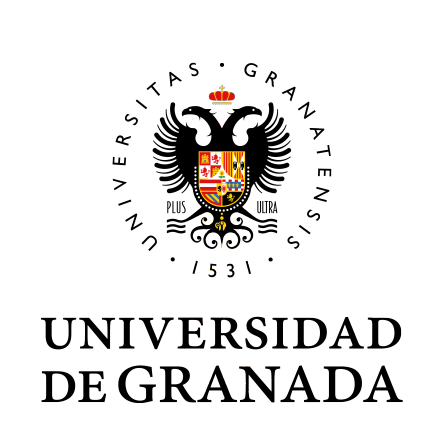
\includegraphics[scale=0.5]{img/ugr.png}\\

\textsc{\Large \asignatura{}\\[0.2cm]}
\textsc{GRADO EN INGENIERÍA INFORMÁTICA}\\[1cm]

\noindent\rule[-1ex]{\textwidth}{1pt}\\[1.5ex]
\textsc{{\Huge \titulo\\[0.5ex]}}
\textsc{{\Large \subtitulo\\}}
\noindent\rule[-1ex]{\textwidth}{2pt}\\[3.5ex]

\end{minipage}

\vspace{0.5cm}

\begin{minipage}{\textwidth}

\centering

\textbf{Autor}\\ {\autor{}}\\[2.5ex]
\textbf{Rama}\\ {Computación y Sistemas Inteligentes}\\[2.5ex]
\vspace{0.3cm}


\includegraphics[scale=0.3]{img/etsiit.jpeg}

\vspace{0.7cm}
\textsc{Escuela Técnica Superior de Ingenierías Informática y de Telecomunicación}\\
\vspace{1cm}
\textsc{Curso 2019-2020}
\end{minipage}
\end{titlepage}

\pagenumbering{arabic}
\tableofcontents
\thispagestyle{empty}				% No usar estilo en la pagina de indice

\newpage

\setlength{\parskip}{1em}

\section{\textsc{Ejercicio sobre filtros básicos}}

\noindent \textbf{USANDO LAS FUNCIONES DE OPENCV}: escribir funciones que implementen los siguientes puntos:

\begin{enumerate}[label=\textbf{\Alph*)}]
	\item \textbf{El cálculo de la convolución de una imagen con una máscara 2D. Usar una Gaussiana 2D (GaussianBlur)
	y máscaras 1D dadas por getDerivKernels). Mostrar ejemplos con distintos tamaños de máscara, valores de
	sigma y condiciones de contorno. Valorar los resultados.}
	\item \textbf{Usar la función Laplacian para el cálculo de la convolución 2D con una máscara normalizada de
	Laplaciana-de-Gaussiana de tamaño variable. Mostrar ejemplos de funcionamiento usando dos tipos de
	bordes y dos valores de sigma: 1 y 3.}
\end{enumerate}

\subsection{Apartado A}

Para realizar todas las pruebas, vamos a utilizar una imágen en blanco y negro. De esta forma, los resultados se podrán
ver de forma más clara. Se puede utilizar cualquiera de las imágenes que se han proporcionado, pero vamos a utilizar
la foto del gato. A continuación se puede ver la imágen en cuestión:

\begin{figure}[H]
\centering
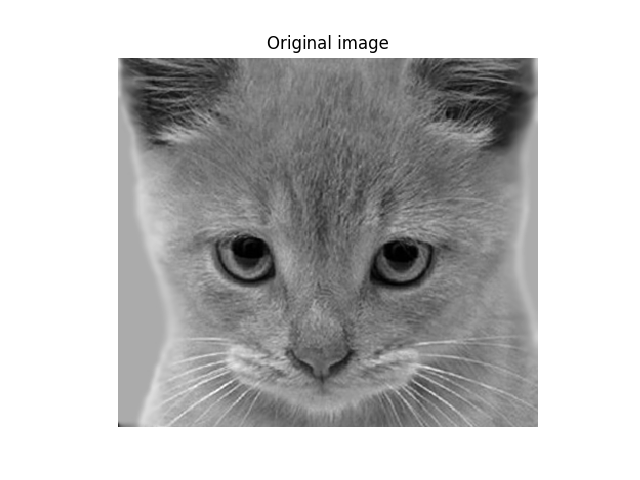
\includegraphics[scale=0.6]{img/cat.png}
\caption{Imágen original del gato en blanco y negro.}
\label{fig:cat}
\end{figure}

Antes de ver cuáles son los resultados y compararlos. Hace falta aclarar algunos puntos:

\begin{itemize}
	\item Cuando se cargan las imágenes, se convierten a \textit{float64}, para así tener más precisión a la hora de
	hacer las posteriores operaciones (aplicar filtros, sumar o restar imágenes, etc.), además de que así no nos limitamos
	a usar solo valores en el rango $[0, 255]$.
	\item Las operaciones para aplicar filtros de OpenCV aplican una correlación. Por tanto, para aplicar una convolución,
	se debe realizar un \textit{flip} del \textit{kernel}; esto es, darle la vuelta en el eje $X$ y en el eje $Y$.
	Como en todos los casos trabajaremos con \textit{kernels} separables, solo será necesario darles la vuelta en un sentido.
	\item Respecto al punto anterior, al trabajar con \textit{kernels} separables, con tal de mejorar la eficiencia,
	se puede aplicar primero el \textit{kernel} del eje $X$ y, sobre el resultado, aplicar el \textit{kernel} en el
	eje $Y$. Esto es mucho más rápido que aplicar directamente un \textit{kernel} 2D sobre la imágen, debido a que el
	número de operaciones es mucho menor.
\end{itemize}

Como en este ejercicio se piden aplicar \textit{kernels} de Gaussiana y de derivada, se han hecho funciones específicas
las cuáles pueden ser consultadas en el código. Estas funciones son \textit{gaussian\_kernel()} y \textit{derivative\_kernel()},
respectivamente. No se va a especificar exactamente lo que hacen debido a que solo obtienen los \textit{kernels} con los
parámetros adecuados (valores de $\sigma$ y tamaño de cada \textit{kernel} para el caso de la Gaussiana, y tamaño del
\textit{kernel} y número de veces que se deriva en cada eje en el caso de la derivada).

Lo que sí que es importante destacar es que estas dos funciones utilizan una común para realizar la convolución. Como se
dijo anteriormente, OpenCV realiza como tal la correlación, pero se puede aplicar una convolución realizando unos pocos cambios.
La función que se puede ver a continuación recibe un \textit{kernel} para cada eje y aplica el filtro mediante la
convolución:

\begin{lstlisting}[caption={Función que aplica un filtro separable.},label={alg:apply-kernel}]
def apply_kernel(img, kx, ky, border):
    """
    Funcion que aplica un kernel separable sobre una imagen,
    realizando una convolucion

    Args:
        img: Imagen sobre la que aplicar el filtro
        kx: Kernel en el eje X
        ky: Kernel en el eje Y
        border: Tipo de borde
    Return:
        Devuelve una imagen filtrada
    """
    # Hacer el flip a los kernels para aplicarlos como una convolucion
    kx_flip = np.flip(kx)
    ky_flip = np.flip(ky)

    # Realizar la convolucion
    conv_x = cv.filter2D(img, cv.CV_64F, kx_flip.T,
    					 borderType=border)
    conv = cv.filter2D(conv_x, cv.CV_64F, ky_flip,
    				   borderType=border)

    return conv
\end{lstlisting}

Como se puede ver, se tiene que hacer un \textit{flip} de los \textit{kernels} para poder aplicar una convolución.
Al aplicar cada \textit{kernel} de forma separada mediante $filter2D$, se consigue una mayor eficiencia (como se ha
mencionado anteriormente). Es importante destacar que primero se aplica el \textit{kernel} sobre el eje de las $X$ y,
sobre el resultado obtenido, se aplica el \textit{kernel} en el eje $Y$. También es importante destacar que, cuando
se aplica el \textit{kernel} sobre el eje $X$, se le pasa la traspuesta del \textit{kernel}. Esto se debe a que
OpenCV proporciona los \textit{kernels} como vectores columnas, y para pasarlo por las filas, necesitamos que sea
un vector fila. Al traponer el vector columna obtenemos, como parece lógico, un vector columna.

Otra cosa muy importante a destacar son los \textit{kernels} que se van a utilizar. Uno de ellos es el \textit{kernel}
Gaussiano, el cuál es simétrico tanto en el eje $X$ como en el $Y$. Al aplicarlo, por tanto, se podría ahorrar la
operación del \textit{flip}, ya que lo va a dejar igual. Sin embargo, debido a que se ha implementado la función
para que sea genérica, se realiza esta operación. El otro \textit{kernel} que se utiliza es el de las derivadas,
que no es más que un \textit{kernel} de Sobel, el cuál combina alisamiento Gaussiano con la derivada.
A diferencia del anterior \textit{kernel}, este no es simétrico, y por tanto, la operación de
\textit{flip} no lo va a dejar igual; por tanto, no puede ser ahorrada en este caso.

Con esto comentado, ya podemos empezar a hablar de los resultados que se han obtenido. Para ello, vamos a comenzar
comentando los resultados que se obtienen para el filtro Gaussiano.

Lo primero que se ha probado es un \textit{kernel} de $5 \times 5$, variando los valores de $\sigma$ para ver cómo cambiaba.
A continuación se pueden ver los resultados:

\begin{figure}[H]
\begin{subfigure}{.5\textwidth}
	\centering
	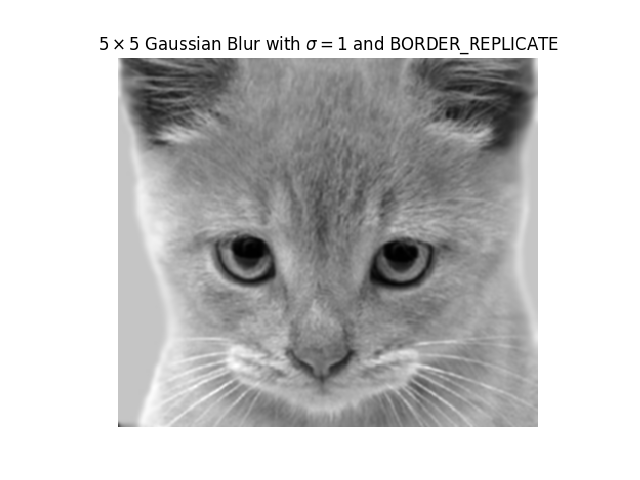
\includegraphics[scale=0.48]{img/gauss-sigma1.png}
	\subcaption{Filtro Gaussiano con $\sigma = 1$.}
	\label{fig:gauss-sigma1}
\end{subfigure}
\begin{subfigure}{.5\textwidth}
	\centering
	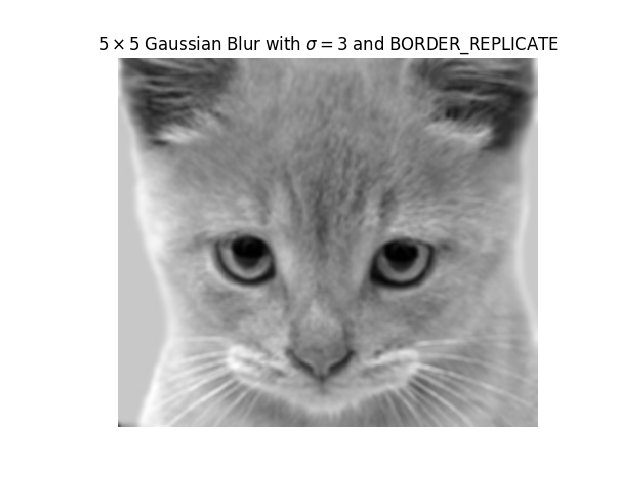
\includegraphics[scale=0.48]{img/gauss-sigma2.png}
	\subcaption{Filtro Gaussiano con $\sigma = 3$.}
	\label{fig:gauss-sigma2}
\end{subfigure}
\caption{Filtro Gaussiano con diferentes tamaños de $\sigma$.}
\label{fig:gauss-sigma}
\end{figure}

Como se puede ver, comparando cualquiera de las imágenes de la figura \ref{fig:gauss-sigma} con \ref{fig:cat}, existen ciertas
diferencias. Podemos ver claramente como al aplicar el filtro Gaussiano se ha perdido cierto detalle, ya que se están
eliminando las frecuencias altas. Además, si comparamos las figuras \ref{fig:gauss-sigma1} y \ref{fig:gauss-sigma2}, podemos
ver que a medida que aumentamos el tamaño de $\sigma$, se van perdiendo más detalles, ya que se emborrona más.

Se ha probado también a variar el tamaño de la máscara, conservando el mismo valor de $\sigma$, para ver qué es lo que sucede.
A continuación, se puede ver lo que se ha obtenido:

\begin{figure}[H]
\begin{subfigure}{.5\textwidth}
	\centering
	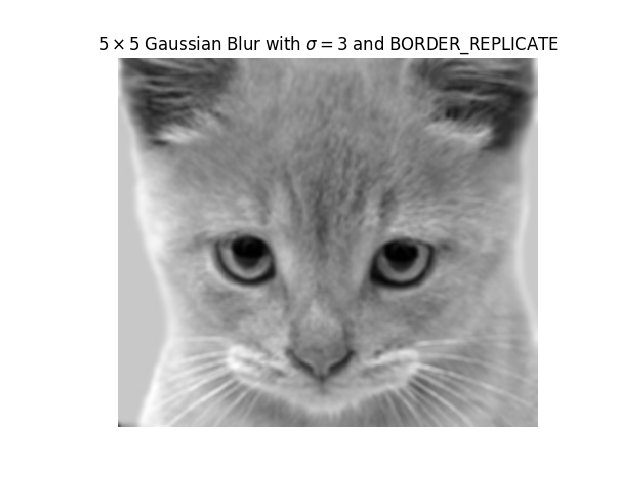
\includegraphics[scale=0.48]{img/gauss-sigma2.png}
	\subcaption{Filtro Gaussiano de tamaño $5 \times 5$.}
	\label{fig:gauss-sigma3}
\end{subfigure}
\begin{subfigure}{.5\textwidth}
	\centering
	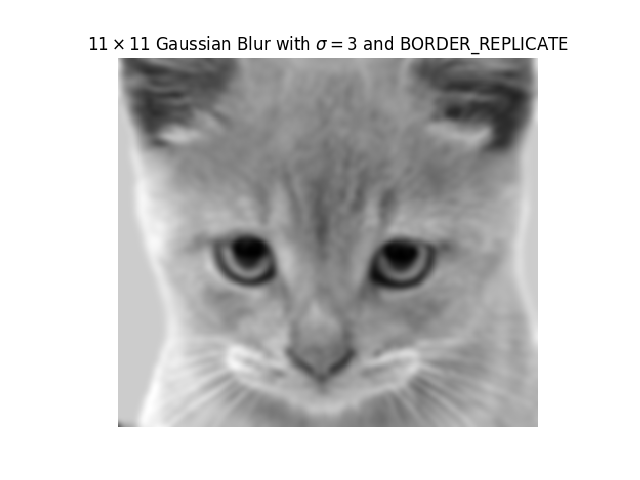
\includegraphics[scale=0.48]{img/gauss-size.png}
	\subcaption{Filtro Gaussiano de tamaño $11 \times 11$.}
	\label{fig:gauss-size1}
\end{subfigure}
\caption{Filtro Gaussiano con diferentes tamaños de \textit{kernel}.}
\label{fig:gauss-size}
\end{figure}

Tal y como se puede ver en la figura \ref{fig:gauss-size}, al modificar el tamaño del \textit{kernel} se han obtenido
diferentes resultados. Esto se debe a que más píxels forman parte de la máscara (como es obvio), y por tanto, se tiene
en cuenta una mayor parte de la Gaussiana. Por tanto, existe cierta dependencia entre esto dos valores (el tamaño del
\textit{kernel} y el valor de $\sigma$). A mayor $\sigma$, mayor tendrá que ser el tamaño de la máscara, para así poder
modelizar mejor el comportamiento de la función con los píxels vecinos. Si no se adaptase el tamaño del \textit{kernel},
se tendría que solo se coge una parte pequeña de la función Gaussiana más cercana al centro, ignorando el comportamiento
de los píxels más lejanos. Tampoco hay que coger un tamaño demasiado grande si el $\sigma$ es pequeño, ya que entonces
habrán muchos píxels que tendrán un valor muy próximo a 0 (aquellos que estén más alejados). En resumen, que hay
escoger de forma proporcional el tamaño del \textit{kernel} y el $\sigma$.

Para ver cómo afecta el tipo de borde a la imágen resultante, se han realizado una serie de pruebas variando el borde
utilizado a la hora de aplicar los \textit{kernels}. Para que los efectos fuesen notables, se ha tenido que escoger un
tamaño de máscara mucho más grande a los utilizados anteriormente. Esto se debe a que con una máscara pequeña no se
puede apreciar muy bien el resultado, debido a que no se coge mucha región fuera de los bordes de la imágen. El tamaño de
la máscara es de $101 \times 101$, permitiendo que se salga lo suficiente de la imágen para ver la influencia. A continuación
se pueden ver los resultados que se han obtenido:

\begin{figure}[H]
\begin{subfigure}{.5\textwidth}
	\centering
	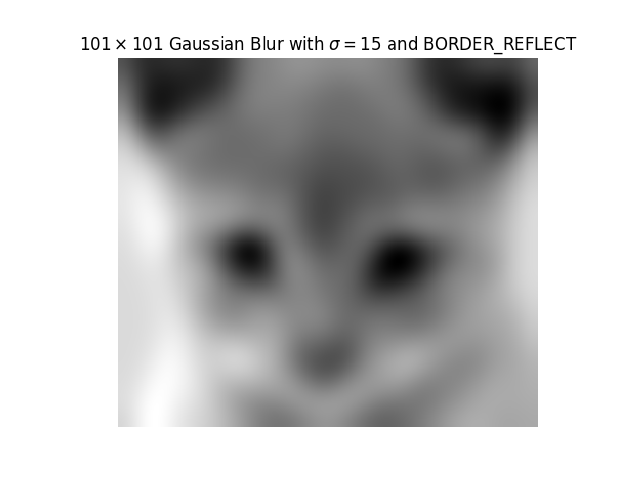
\includegraphics[scale=0.47]{img/gauss-border1.png}
	\subcaption{Borde reflejando la imágen.}
	\label{fig:gauss-border1}
\end{subfigure}
\begin{subfigure}{.5\textwidth}
	\centering
	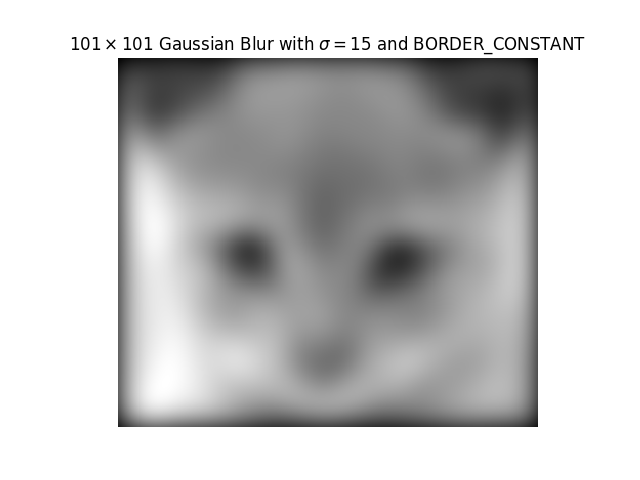
\includegraphics[scale=0.47]{img/gauss-border2.png}
	\subcaption{Borde constante.}
	\label{fig:gauss-border2}
\end{subfigure}
\end{figure}
\begin{figure}[H]\ContinuedFloat
\begin{subfigure}{\textwidth}
	\centering
	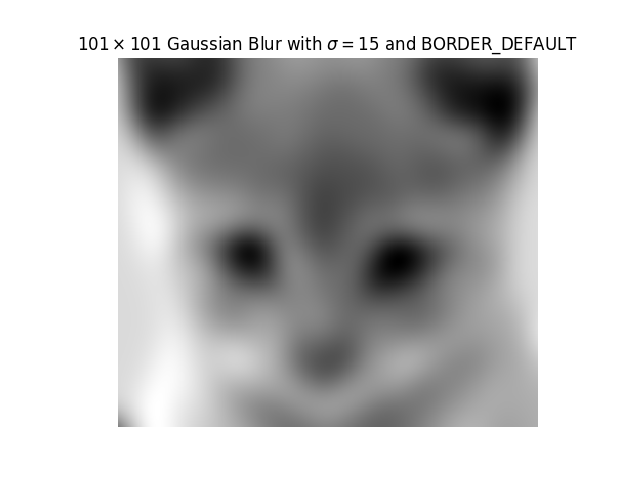
\includegraphics[scale=0.5]{img/gauss-border3.png}
	\subcaption{Borde por defecto (reflejado sin contar el primer píxel).}
	\label{fig:gauss-border3}
\end{subfigure}
\caption{Filtro Gaussiano con diferentes tipos de bordes.}
\label{fig:gauss-borders}
\end{figure}

Como se puede ver, existen ciertas diferencias dependiendo de qué tipo de borde se escoja. Si comparamos las figuras
\ref{fig:gauss-border1} y \ref{fig:gauss-border3} con la figura \ref{fig:gauss-border2}, se puede ver claramente que
los resultados no son los mismos, ya que en este último caso se utiliza un valor constante para las partes más allá
de los bordes de las imágenes. Por tanto, la imágen queda como si estuviese enmarcada.

Las diferencias entre las figuras \ref{fig:gauss-border1} y \ref{fig:gauss-border3} son mucho más sutiles, pero notables.
Se puede ver como por ejemplo en la figura \ref{fig:gauss-border3} la esquina inferior izquierda es más oscura, mientras
que en la figura \ref{fig:gauss-border1} es más clara. Aunque los dos tipos de borde reflejen la imágen, la forma en la
que lo hacen es distinto. $BORDER\_DEFAULT$ no considera el píxel del borde, mientras que $BORDER\_REFLECT$ sí que lo hace.
Todo esto se puede ver mejor explicado aquí. %INSERTAR REFERENCIA

Por último, y antes de pasar al \textit{kernel} de derivada, se ha probado a variar el $\sigma$ que se ha aplicado en cada
eje, manteniendo constante el tamaño del \textit{kernel}. A continuación se pueden ver cuáles han sido los rsultados obtenidos:

\begin{figure}[H]
\begin{subfigure}{.5\textwidth}
	\centering
	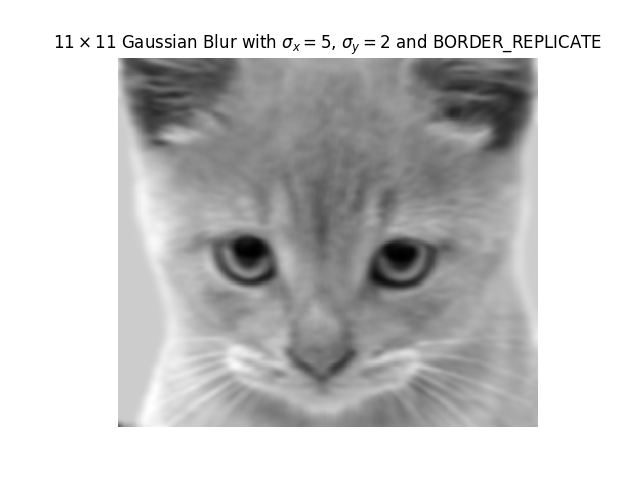
\includegraphics[scale=0.45]{img/gauss-diff1.png}
	\subcaption{Filtro Gaussiano con $\sigma_x = 5$ y $\sigma_y = 2$.}
	\label{fig:gauss-diff1}
\end{subfigure}
\begin{subfigure}{.5\textwidth}
	\centering
	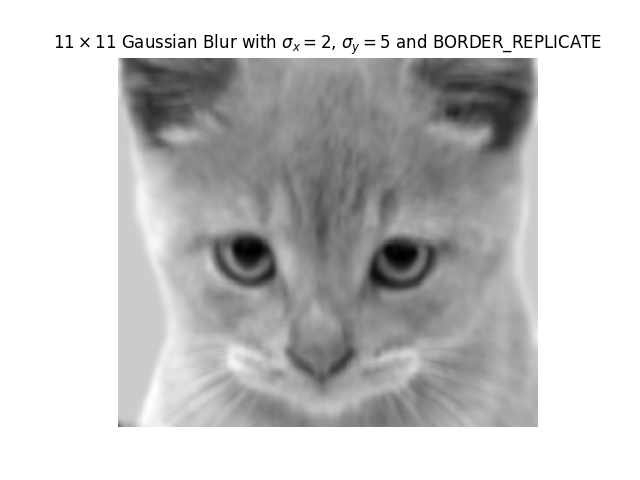
\includegraphics[scale=0.45]{img/gauss-diff2.png}
	\subcaption{Filtro Gaussiano con $\sigma_x = 2$ y $\sigma_y = 5$.}
	\label{fig:gauss-diff2}
\end{subfigure}
\caption{Filtro Gaussiano variando el $\sigma$ en cada eje.}
\label{fig:gauss-diff}
\end{figure}

Como se puede ver claramente, hay diferencias, debido a que el alisamiento solo se ha hecho en uno de los ejes en
vez de en los dos. Se puede ver como en la figura \ref{fig:gauss-diff1} el pelo de la frente del gato parece que
va hacia la derecha, mientras que en la figura \ref{fig:gauss-diff2} el pelo de la frente parece que va hacia abajo.
Además, en esta segunda imágen se puede ver como los bigotes se han emborronado más que en el primer caso, donde
son más apreciables.

Con esto ya comentado, pasemos a hablar del \textit{kernel} de las derivadas. Lo primero que podemos hacer es ver
qué influencia tiene la derivada dependiendo del eje sobre el que se aplique y según el número de veces que se derive
en cada uno de los ejes. Para ello, vamos a probar la primera y la segunda derivada en cada uno de los ejes de forma
separada (esto es, que no derivaremos a la vez). A continuación se pueden ver los resultados:

\begin{figure}[H]
\begin{subfigure}{.5\textwidth}
	\centering
	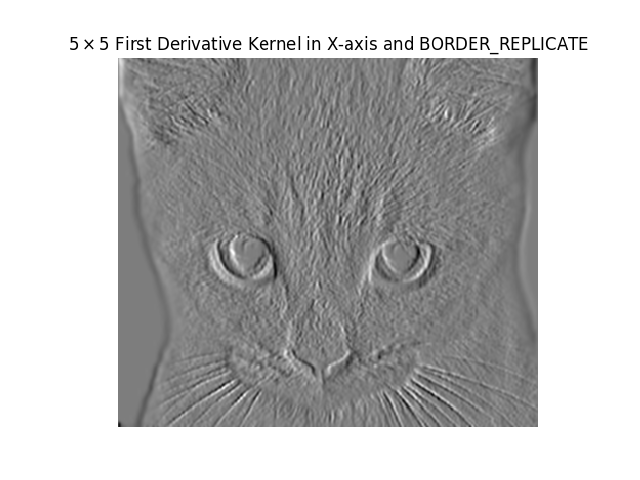
\includegraphics[scale=0.45]{img/der-x1.png}
	\subcaption{Filtro de primera derivada en el eje $X$.}
	\label{fig:der-x1}
\end{subfigure}
\begin{subfigure}{.5\textwidth}
	\centering
	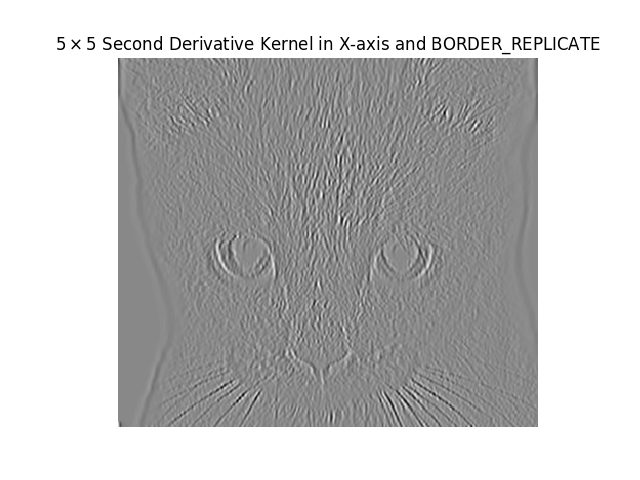
\includegraphics[scale=0.45]{img/der-x2.png}
	\subcaption{Filtro de segunda derivada en el eje $X$.}
	\label{fig:der-x2}
\end{subfigure}
\end{figure}
\begin{figure}[H]\ContinuedFloat
\begin{subfigure}{.5\textwidth}
	\centering
	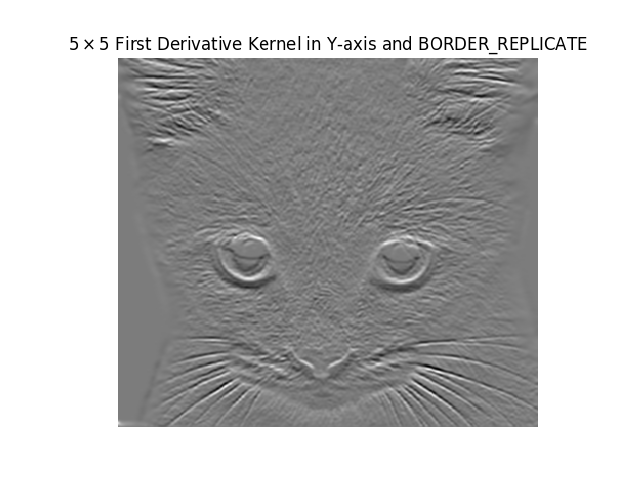
\includegraphics[scale=0.45]{img/der-y1.png}
	\subcaption{Filtro de primera derivada en el eje $Y$.}
	\label{fig:der-y1}
\end{subfigure}
\begin{subfigure}{.5\textwidth}
	\centering
	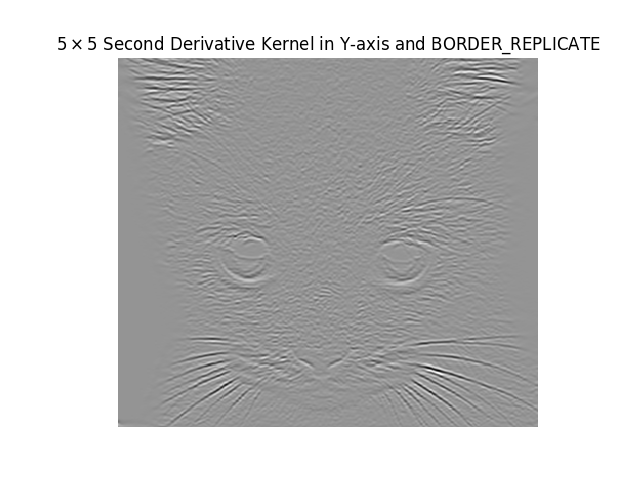
\includegraphics[scale=0.45]{img/der-y2.png}
	\subcaption{Filtro de segunda derivada en el eje $Y$.}
	\label{fig:der-y2}
\end{subfigure}
\caption{Filtro de derivada variando el número de diferenciaciones en cada eje.}
\label{fig:der}
\end{figure}

Al pasarlo por el eje $X$, como se puede ver en las figuras \ref{fig:der-x1} y \ref{fig:der-x2}, se puede ver que se van
quedando aquellos bordes verticales, ya que los horizontales se ven muy poco o nada, como es por ejemplo el caso del pelo
de las orejas, el cuál casi no se ve, o algunos de los bigotes. En cambio, al pasarlo por el eje $Y$, tal y como se
puede ver en las figuras \ref{fig:der-y1} y \ref{fig:der-y2}, se van quedando aquellos bordes que horizontales.
Se puede ver que el pelo en las orejas se puede ver mejor, además de que algunos de los bigote están mejor definidos
que en el caso anterior. Lo único que se va perdiendo son los bordes del gato como tal, haciendo que, a medida que se
va derivando más en el eje $Y$, se distinga menos donde empieza el gato y donde está el fondo.

También se ha decidido estudiar qué efecto tiene pasar el \textit{kernel} de las derivadas tanto en el eje $X$ como en
el $Y$ a la vez, ya que la función $getDerivKernel$ permite especificar el número de diferenciaciones a realizar en cada
eje. Los resultados que se han obtenido son los siguientes:

\begin{figure}[H]
\begin{subfigure}{.5\textwidth}
	\centering
	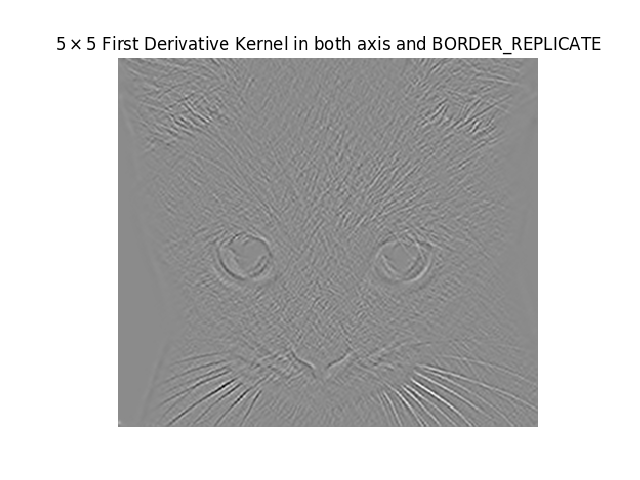
\includegraphics[scale=0.37]{img/der-xy1.png}
	\subcaption{Filtro de primera derivada en ambos ejes.}
	\label{fig:der-xy1}
\end{subfigure}
\begin{subfigure}{.5\textwidth}
	\centering
	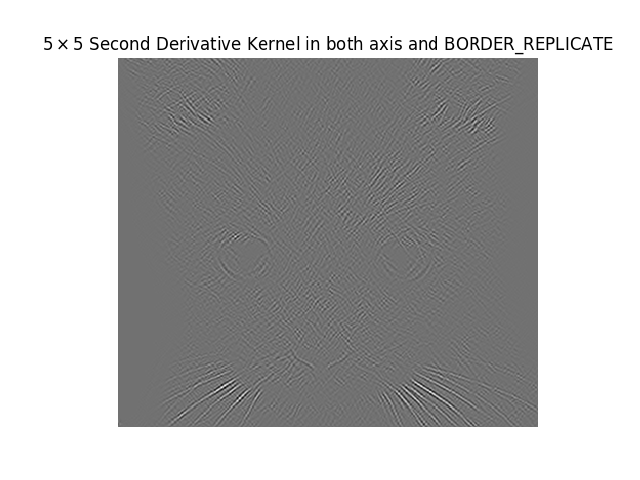
\includegraphics[scale=0.37]{img/der-xy2.png}
	\subcaption{Filtro de segunda derivada en ambos ejes.}
	\label{fig:der-xy2}
\end{subfigure}
\caption{Filtro de derivada variando el número de diferenciaciones en los dos ejes.}
\label{fig:der-xy}
\end{figure}

A diferencia de lo que se ve en la figura \ref{fig:der}, en la figura \ref{fig:der-xy} se observa que aquellos bordes que
destacan más son los que están en diagonal (es decir, una combinación de los dos ejes). Los horizontales y los verticales
casi no se notan, como por ejemplo es el caso de los contornos del gato, ya que aquí es incluso más difícil o casi imposible
distinguir donde empieza el gato y donde empieza el fondo.

Ahora, tal y como hicimos antes, pasemos a ver qué pasa si mantenemos el número de diferenciaciones constante y aumentamos
el tamaño del \textit{kernel}. Para ello, vamos a establecer que en todos los casos se obtiene la primera derivada en el eje
$X$. Los resultados de estas variaciones del tamaño del \textit{kernel} se pueden ver a continuación:

\begin{figure}[H]
\begin{subfigure}{.5\textwidth}
	\centering
	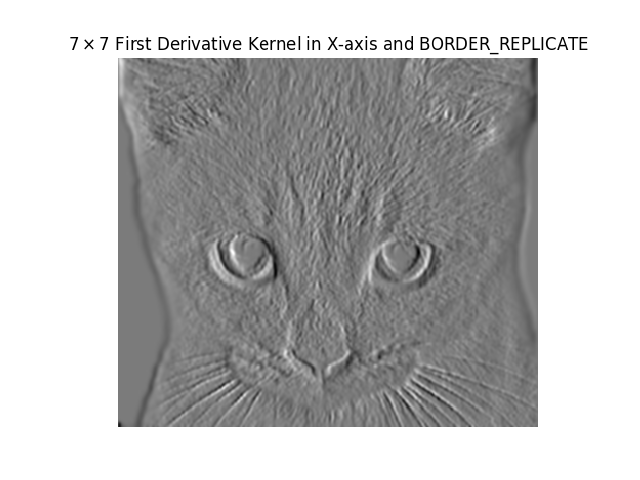
\includegraphics[scale=0.46]{img/der-size1.png}
	\subcaption{Filtro de tamaño $7 \times 7$.}
	\label{fig:der-size1}
\end{subfigure}
\begin{subfigure}{.5\textwidth}
	\centering
	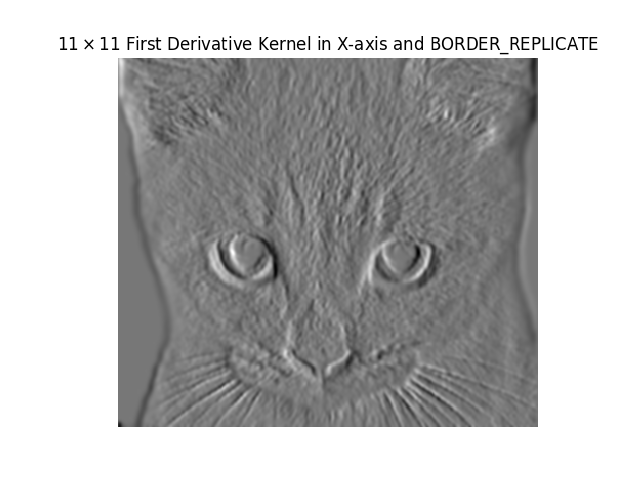
\includegraphics[scale=0.46]{img/der-size2.png}
	\subcaption{Filtro de tamaño $11 \times 11$.}
	\label{fig:der-size2}
\end{subfigure}
\begin{subfigure}{\textwidth}
	\centering
	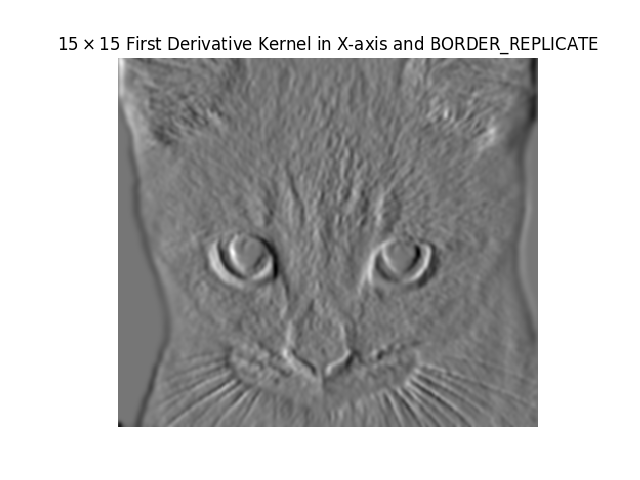
\includegraphics[scale=0.46]{img/der-size3.png}
	\subcaption{Filtro de tamaño $15 \times 15$.}
	\label{fig:der-size3}
\end{subfigure}
\caption{Filtro de primera derivada en el eje $X$ variando el tamaño del \textit{kernel}.}
\label{fig:der-size}
\end{figure}

Como resultado más obvio, se puede ver que a medida que va aumentando el tamaño del \textit{kernel}, se va emborronando más
la imágen. Esto se debe a que uno de los \textit{kernels} de Sobel hace un suavizado, de forma que se va eliminando el ruido.
A mayor tamaño del \textit{kernel}, más se va a emborronar. Por tanto, aquellos bordes muy finos se van a ir perdiendo. Por
ejemplo, si comparamos la figura \ref{fig:der-size1} con la figura \ref{fig:der-size3}, podemos ver que los bordes o contornos
que se pueden ver en la primera figura en la frente del gato han ido desapariciendo o haciéndose menos notables en esta última.
De esta forma, aumentar el tamaño del \textit{kernel} parece que solo nos aporta más suaviazado. Un tamaño de \textit{kernel}
relativamente pequeño es suficiente para extraer los contornos.

Por último, vamos a ver como variando el tipo de borde cambia la imágen que obtenemos. Para ello, tal y como hicimos antes, vamos
a fijar un tamaño de \textit{kernel} relativamente grande para poder apreciar el efecto del borde. En este caso, estamos limitados
a un tamaño máximo de 31, ya que OpenCV no permite obtener más. Por tanto, vamos a usar este tamaño de \textit{kernel} a la hora
de variar los bordes, ya que se ha considerado el más adecuado para la labor. A continuación se pueden ver los resultados:

\begin{figure}[H]
\begin{subfigure}{.5\textwidth}
	\centering
	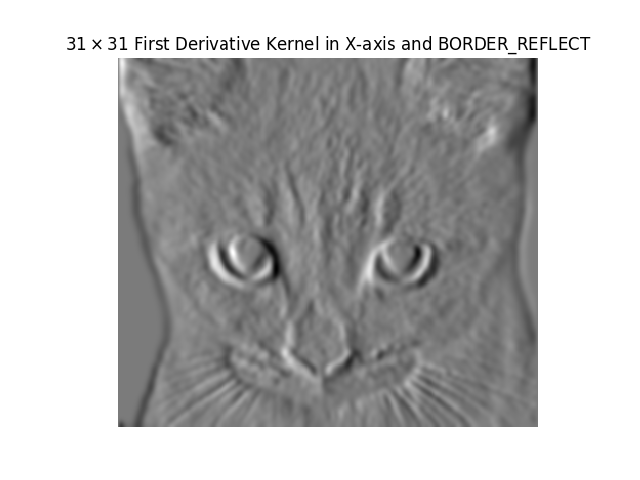
\includegraphics[scale=0.44]{img/der-border1.png}
	\subcaption{Borde reflejando la imágen.}
	\label{fig:der-border1}
\end{subfigure}
\begin{subfigure}{.5\textwidth}
	\centering
	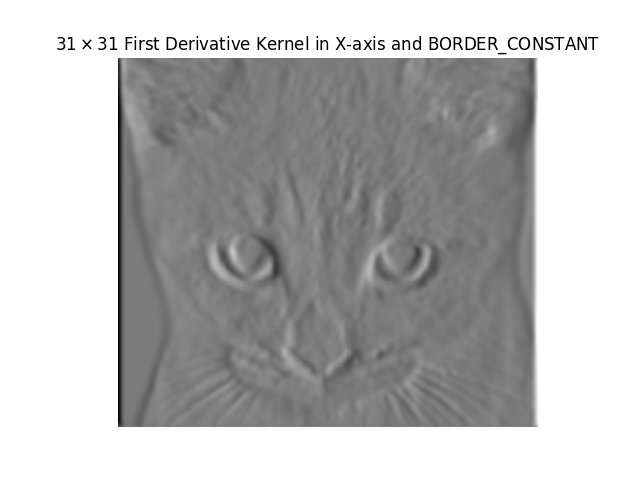
\includegraphics[scale=0.44]{img/der-border2.png}
	\subcaption{Borde constante.}
	\label{fig:der-border2}
\end{subfigure}
\begin{subfigure}{\textwidth}
	\centering
	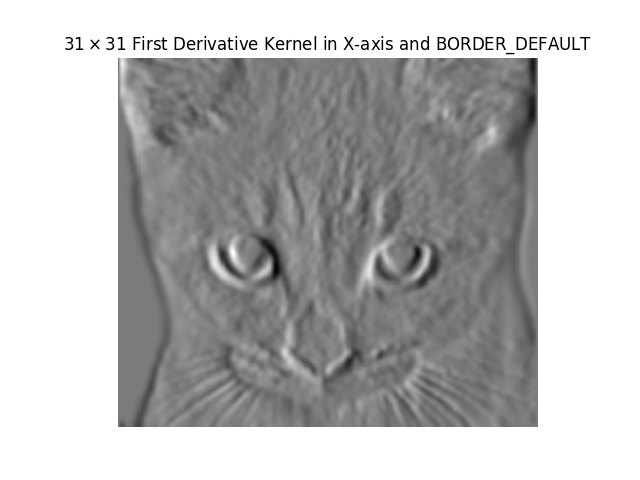
\includegraphics[scale=0.44]{img/der-border3.png}
	\subcaption{Borde por defecto (reflejado sin contar el primer píxel).}
	\label{fig:der-border3}
\end{subfigure}
\caption{Filtro de primera derivada en el eje $X$ variando el tipo de borde.}
\label{fig:der-border}
\end{figure}

En este caso, sucede algo parecido a lo que se podía ver en la figura \ref{fig:gauss-borders}. Podemos ver que
la figura más diferente de todas es la figura \ref{fig:der-border2}. Sin embargo, no parece que haya mucha diferencia
destacable o notable entre las figuras \ref{fig:der-border1} y \ref{fig:der-border3}, con lo cuál podríamos decir que
permiten obtener un resultado más o menos parecido, sin demasiadas diferencias. Parece que en este caso el tipo
de borde que más afecta es el constante, aquél en el que se supone un valor constante para todos los píxels fuera de la imágen.
Por tanto, si utilizamos cualquier otro tipo de borde no notaríamos mucha diferencia, lo cuál no sucedía en el caso del
filtro Gaussiano, ya que sí que había algunas diferencias, aunque fuesen muy pocas.

\subsection{Apartado B}

Antes de analizar los resultados, vamos a comentar brevemente cómo es la función de la Laplaciana de Gaussiana. El código
es el que se puede ver a continuación:

\begin{lstlisting}[caption={Función que aplica una Laplaciana de Gaussiana.},label={alg:log-kernel}]
def log_kernel(img, ksize, sigma_x, sigma_y, border):
    """
    Funcion que aplica un kernel LoG (Laplacian of Gaussian) sobre una imagen.

    Args:
        img: Imagen sobre la que aplicar el kernel
        ksize: Tamaño del kernel Gaussiano y Laplaciano
        sigma_x: Valor de sigma en el eje X de la Gaussiana
        sigma_y: Valor de sigma en el eje Y de la Gaussiana
        border: Tipo de borde
    Return:
        Devuelve una imagen sobre la que se ha aplicado un filtro LoG
    """

    # Aplicar filtro Gaussiano
    gauss = gaussian_kernel(img, ksize, ksize, sigma_x, sigma_y, border)
    
    # Obtener los filtros de derivada segunda en cada eje, aplicados sobre
    # el filtro Gaussiano
    dx2 = derivative_kernel(gauss, 2, 0, ksize, border)
    dy2 = derivative_kernel(gauss, 0, 2, ksize, border)
    
    # Combinar los filtros de derivadas y obtener Laplaciana de Gaussiana
    laplace = dx2 + dy2

    return laplace
\end{lstlisting}

Lo primero que se hace es aplicar un filtro de Gaussiana sobre la imágen de entrada. Al ser éste un filtro de paso bajo, las
altas frecuencias (y el ruido) se eliminan, quedando una imágen más suavizada. Después, sobre el resultado de aplicar el
filtro, se obtienen los filtros de segunda derivada para cada eje. Lo único que hay que hacer al final es combinar la
segunda derivada en el eje $X$ y la segunda derivada en el eje $Y$. Estos dos últimos pasos (diferenciación y suma) se
han seguido según la fórmula de la Laplaciana, la cuál es:

\begin{equation}
\texttt{dst} = \Delta \texttt{src} = \frac{\partial^2 \texttt{src}}{\partial x^2} + \frac{\partial^2 \texttt{src}}{\partial y^2}
\end{equation}

Hay que tener en cuenta que el filtro de derivada tiene una parte que es también un filtro de alisamiento. Por tanto, al
aplicarlo junto con la Gaussiana, se alisa más la imágen. Esto nos hace replantearnos el uso del filtro Gaussiano del
principio. Sin embargo, también hay que considerar que el alisamiento de la derivada por sí solo no es muy grande. Por consiguiente,
vamos a dejar el filtro Gaussiano del principio, aunque se acabe alisndo algo más de lo que se debe.

Una vez comentado esto, vamos a ver cuáles son los resultados que se han obtenido. Lo primero que se ha probado es a variar
el tamaño del $\sigma$ utilizado, utilizando en ambos casos un \textit{kernel} de $5 \times 5$. Los resultados son los que
se pueden ver a continuación:

\begin{figure}[H]
\begin{subfigure}{.5\textwidth}
	\centering
	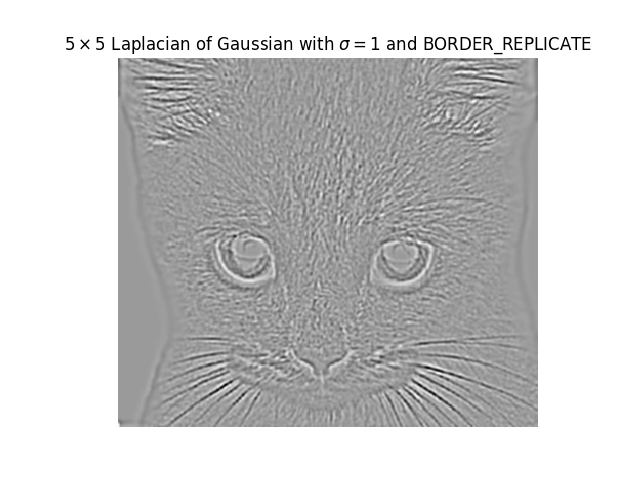
\includegraphics[scale=0.45]{img/laplacian-sigma1.png}
	\subcaption{Filtro con $\sigma = 1$.}
	\label{fig:laplacian-sigma1}
\end{subfigure}
\begin{subfigure}{.5\textwidth}
	\centering
	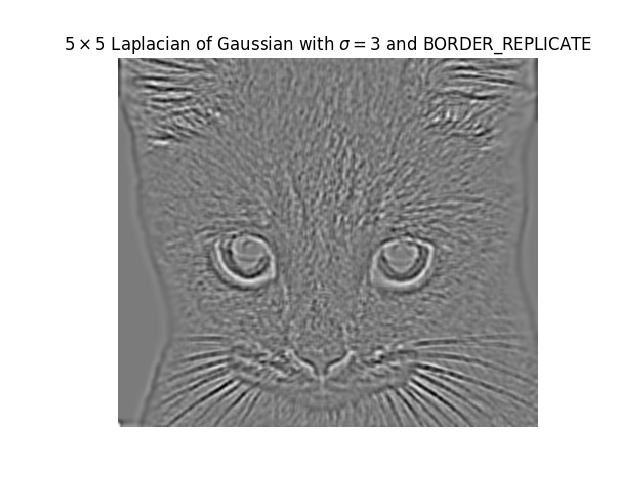
\includegraphics[scale=0.45]{img/laplacian-sigma2.png}
	\subcaption{Filtro con $\sigma = 3$.}
	\label{fig:laplacian-sigma2}
\end{subfigure}
\caption{Filtro de Laplaciana de Gaussiana con diferentes valores de $\sigma$.}
\label{fig:laplacian-sigma}
\end{figure}

Como se puede ver, al aumentar el tamaño de $\sigma$ se obtiene un mayor suavizado (debido a la Gaussiana), además de que
la imágen pierde intensidad debido a esto mismo. Además, se puede ver como los bordes son más gruesos. En la figura
\ref{fig:laplacian-sigma1} los bordes en las orejas y los bigotes son mucho más finos que los que se pueden ver en la
figura \ref{fig:laplacian-sigma2}. Esto se debe a lo comentado anteriormente: un mayor emoborronamiento.

Como también se ha pedido, se ha probado a modificar el tipo de borde utilizado para ver qué efecto tiene sobre la imágen
resultante. Para ello, tal y como se ha hecho anteriormente se ha utilizado un \textit{kernel} de mayor tamaño, concretamente
de 31. De esta forma, el efecto sería más apreciable. Se ha utilizado el mismo borde que se puede ver en la figura
\ref{fig:laplacian-sigma}, y otro más. Además, se ha fijado un $\sigma = 3$ para los dos casos. Los resultados se pueden ver
a continuación:

\begin{figure}[H]
\begin{subfigure}{.5\textwidth}
	\centering
	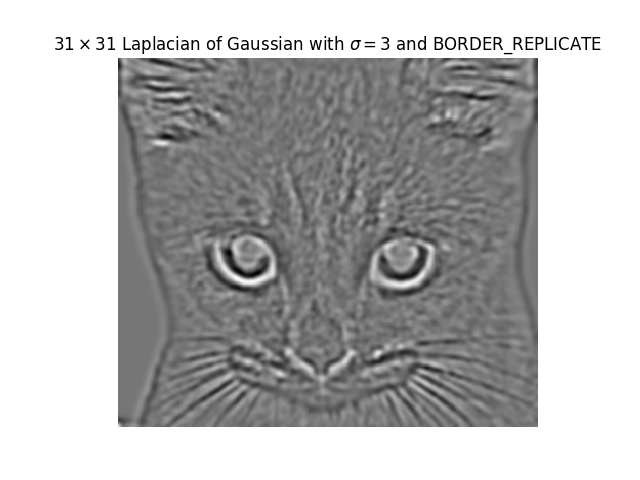
\includegraphics[scale=0.45]{img/laplacian-border1.png}
	\subcaption{Filtro replicando el píxel del borde.}
	\label{fig:laplacian-border1}
\end{subfigure}
\begin{subfigure}{.5\textwidth}
	\centering
	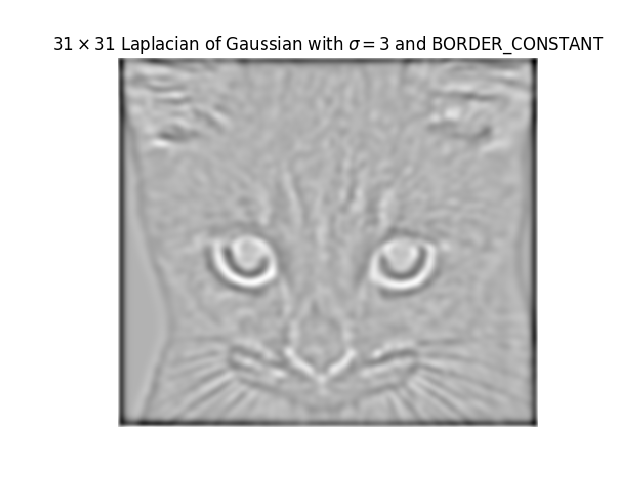
\includegraphics[scale=0.45]{img/laplacian-border2.png}
	\subcaption{Filtro con borde constante.}
	\label{fig:laplacian-border2}
\end{subfigure}
\caption{Filtro de Laplaciana de Gaussiana con diferentes valores de $\sigma$.}
\label{fig:laplacian-border}
\end{figure}

Claramente se pueden apreciar las diferencias. Se puede ver que la imágen que se ve en la figura \ref{fig:laplacian-border2}
parece estar enmarcada, debido a que tiene los píxels de color negro en los bordes. Además, tiene una mayor intensidad que
la que se puede ver en la figura \ref{fig:laplacian-border1}, aunque el precio a pagar ha sido que se ha perdido demasiado
detalle por el camino.

\newpage

\section{\textsc{Ejercicio sobre pirámides y detección de regiones}}

\noindent \textbf{IMPLEMENTAR} funciones para las siguiente tareas:

\begin{enumerate}[label=\textbf{\Alph*)}]
	\item \textbf{Una función que genere una representación en pirámide Gaussiana de 4 niveles de una
	imagen. Mostrar ejemplos de funcionamiento usando bordes y justificar la elección de los parámetros.}
	\item \textbf{Una función que genere una representación en pirámide Laplaciana de 4 niveles de una imagen.
	Mostrar ejemplos de funcionamiento usando bordes.}
	\item \textbf{Construir un espacio de escalas Laplaciano para implementar la búsqueda de regiones usando el siguiente
	algoritmo:}
	\begin{enumerate}[label=\textbf{\alph*.}]
		\item Fijar sigma
		\item Repetir para N escalas
		\begin{enumerate}[label=\roman*.]
			\item Filtrar la imagen con la Laplaciana-Gaussiana normalizada en escala
			\item Guardar el cuadrado de la respuesta para el actual nivel del espacio de escalas
			\item Incrementar el valor de sigma por un coeficiente k.( 1.2-1.4)
		\end{enumerate}
		\item Realizar supresión de no-máximos en cada escala
		\item Mostrar las regiones encontradas en sus correspondientes escalas. Dibujar círculos con radio proporcional a
		la escala.
	\end{enumerate}
\end{enumerate}

\subsection{Apartado A}

Para crear la pirámide Gaussiana, se ha utilizado la siguiente función:

\begin{lstlisting}[caption={Función que crea una priámide Gaussiana.},label={alg:guassian-pyramid}]
def gaussian_pyramid(img, ksize, sigma_x, sigma_y, border, N=4):
    """
    Funcion que devuelve una piramide Gaussiana de tamaño N

    Args:
        img: Imagen de la que extraer la piramide
        ksize: Tamaño del kernel
        sigma_x: Valor de sigma en el eje X
        sigma_y: Valor de sigma en el eje Y
        border: Tipo de borde a utilizar
        N: Numero de imagenes que componen la piramide (default 4)

    """
    # Inicializar la piramide con la primera imagen
    gaussian_pyr = [img]

    for i in range(1, N):
        # Obtener el elemento anterior de la piramide Gaussiana
        prev_img = np.copy(gaussian_pyr[i - 1])

        # Aplicar Gaussian Blur
        gauss = gaussian_kernel(prev_img, ksize, ksize, sigma_x, sigma_y, border)

        # Reducir el tamaño de la imagen a la mitad
        down_sampled_gauss = gauss[1::2, 1::2]

        # Añadir imagen a la piramide
        gaussian_pyr.append(down_sampled_gauss)


    return gaussian_pyr
\end{lstlisting}

Entender el funcionamiento del código es bastante directo, pero por si acaso, vamos a describir brevemente lo que hace. Esta
función crea la pirámide Gaussiana de $N$ niveles (contando como primer nivel la imágen original). Por tanto, la imágen
resultante estará compuesta de la imágen original y las $N - 1$ reducciones de la imágen original. Para obtener la siguiente
imágen de la pirámide, simplemente basta con coger el nivel anterior, aplicarle un filtro Gaussiano y reducir su tamaño a la
mitad, y posteriormente guardar el resultado. Todo esto se corresponde con la parte del bucle, la cuál se realiza $N - 1$ veces.

Lo más importante a destacar es el escalado de la imágen, el cuál puede ser visto en línea 25. Lo que se hace es coger todas las
filas y columnas pares, ignorando las impares. De esta forma, si se escala una imágen que tenga alguna de sus dimensiones (o bien
el número de filas o bien el número de columnas) impar, en el siguiente nivel estos valores serán pares. De la otra forma, si
cogíesemos las filas y columnas impares, esto no se daría, ya que si alguna de las dimensiones fuese impar, en el siguiente
nivel también lo sería. Es preferible trabajar con dimensiones pares, ya que así se pierde menos información al tomar una
muestra de su espacio.

Una vez habiendo comentado esto, vamos a ver algún ejemplo de pirámide Gaussiana:

\begin{figure}[H]
\centering
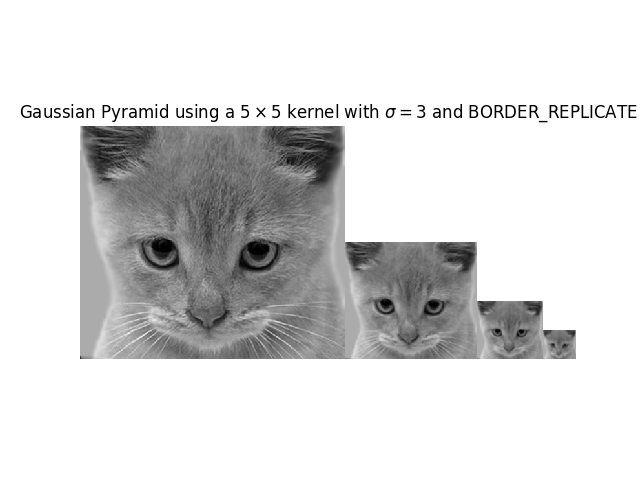
\includegraphics[scale=0.6]{img/gauss-pyr-1.png}
\caption{Pirámide Gaussiana utilizando un \textit{kernel} $5 \times 5$ en cada nivel con $\sigma = 3$.}
\label{fig:gauss-pyr-1}
\end{figure}

Tal y como se puede ver en la figura \ref{fig:gauss-pyr-1} se crea una pirámide en la que al reducir el tamaño de la
imágen no se pierde demasiado detalle, ya que la figura del gato sigue siendo distinguible en cada nivel.

Se ha elegido un tamaño de \textit{kernel} de $5 \times 5$ con un $\sigma = 3$ en cada eje porque es una máscara no
muy grande y que aplica un suavizado suficiente para cada nivel, es decir, que ni aplica demasiado ni demasiado poco, tal
y como se comprobó en la figura \ref{fig:gauss-sigma}. Otro motivo importante es que, cuantos más niveles tenga la pirámide,
más pequeña se irá haciendo la imágen, y por tanto, no interesa tener una máscara enorme con un sigma muy grande, ya que se
va a emborronar demasiado. Se ha elegido un borde de tipo replicado porque en general no modifica mucho la imágen de salida.
En este caso, la pirámide es de 4 niveles; es decir, $N=4$, tal y como se ha pedido.

Para ver si cambiando el tipo de borde obtenemos algo diferente, se ha probado a utilizar un borde constante.
El resto de parámetros se han dejado igual. A continuación se pueden ver los resultados:

\begin{figure}[H]
\centering
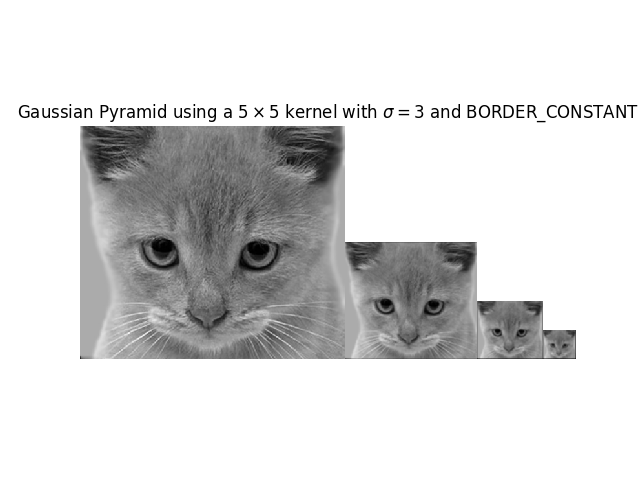
\includegraphics[scale=0.6]{img/gauss-pyr-2.png}
\caption{Pirámide Gaussiana con borde constante.}
\label{fig:gauss-pyr-2}
\end{figure}

Se puede ver que existen unas pequeñas diferencias si lo comparamos con la figura \ref{fig:gauss-pyr-1}. En los niveles
más altos, no tiene mucha influencia el haber cambiado el tipo de borde, pero a medida que la imágen se va haciendo más pequeña,
se pueden ver como comienzan a aparecer los recuadros negros, tal y como hemos visto anteriormente en la figura
\ref{fig:gauss-border2}. A parte de esto, no hay muchas más diferencias apreciables, lo cuál se puede deber a
que el tamaño del \textit{kernel} no es tan grande a como lo era antes.

\subsection{Apartado B}

Para crear la pirámide Laplaciana, se ha utilizado la siguiente función:

\begin{lstlisting}[caption={Función que crea una pirámide Laplaciana.},label={alg:laplacian-pyramid}]
def laplacian_pyramid(img, ksize, sigma_x, sigma_y, border, N=4):
    """
    Funcion que crea una piramide Laplaciana de una imagen

    Args:
        img: Imagen de la que crar la piramide
        ksize: Tamaño del kernel
        sigma_x: Valor de sigma en el eje X
        sigma_y: Valor de sigma en el eje Y
        border: Tipo de borde
        N: Numero de componentes de la piramide. El nivel Gaussiano (ultimo)
           no esta incluido(default 4)
    Return:
        Devuelve una lista que contiene las imagenes que forman la piramide
    """

    # Obtener piramide Gaussiana de un nivel mas
    gaussian_pyr = gaussian_pyramid(img, ksize, sigma_x, sigma_y, border, N+1)

    # Crear la lista que contendra la piramide Laplaciana
    # Se inserta el ultimo elemento de la piramide Gaussiana primero
    laplacian_pyr = [gaussian_pyr[-1]]

    # Recorrer en orden inverso la piramide Gaussiana y generar la Laplaciana
    for i in reversed(range(1, N+1)):
        # Obtener la imagen actual y la anterior
        current_img = gaussian_pyr[i]
        previous_img = gaussian_pyr[i - 1]

        # Hacer upsampling de la imagen actual
        upsampled_img = np.repeat(current_img, 2, axis=0)
        upsampled_img = np.repeat(upsampled_img, 2, axis=1)

        # Si falta una fila, copiar la ultima
        if upsampled_img.shape[0] < previous_img.shape[0]:
            upsampled_img = np.vstack([upsampled_img, upsampled_img[-1]])

        # Si falta una fila, copiar la ultima
        if upsampled_img.shape[1] < previous_img.shape[1]:
            upsampled_img = np.hstack([upsampled_img, upsampled_img[:, -1].reshape(-1, 1)])

        # Pasar un Gaussian Blur a la imagen escalada para intentar suavizar el efecto de las
        # filas y las columnas repetidas
        upsampled_gauss = gaussian_kernel(upsampled_img, ksize, ksize, sigma_x, sigma_y, border)

        # Restar la imagen orignal de la escalada para obtener detalles
        diff_img = previous_img - upsampled_gauss

        # Guardar en la piramide
        laplacian_pyr.insert(0, diff_img)


    return laplacian_pyr
\end{lstlisting}

Esta vez, a diferencia de lo que se podía ver en el código \ref{alg:guassian-pyramid}, el código puede que no
sea tan sencillo de entender. Por tanto, vamos a intentar explicar de manera breve y simple qué es lo que hace.

Para generar una pirámide Laplaciana de $N$ niveles, lo más fácil es partir de una pirámide Gaussiana de $N + 1$ niveles
(el último será la imágen más pequeña, la cuál contendrá las bajas frecuencias, a diferencia del resto de imágenes
de la priámide). Comenzando desde esta imágen más pequeña, se realiza un escalado hacia arriba para que tenga las mismas
dimensiones de la imágen del nivel anterior. Este escalado se realiza replicando todas las filas y columnas. Sobre este
escalado se aplica un filtro Gaussiano para suavizar la imágen, ya que contiene información redundante e interesa
modificar los píxels para que se tenga en cuenta el entorno. Finalmente, se resta la imágen escalada y suavizada
al anterior nivel de la pirámide Gaussiana para obtener las altas frecuencias, y se almacena esta información.

El proceso de escalado o \textit{upsampling} es muy importante, y se debe destacar la forma en la que se hace. Este
procedimiento se puede ver en las líneas 31-40. Como se dijo anteriormente, se replican las filas y columnas, insertándolas
al lado de las originales. Este es el procedimiento más sencillo que se puede realizar, ya que se duplica el tamaño de la
imágen con valores ``válidos''. Sin embargo, aparece un pequeño problema: puede suceder que alguna de las dimensiones
de la imágen del nivel anterior sea impar. Como las imágenes deben tener el mismo tamaño para poder obtener las altas
frecuencias, lo que se ha decidido es añadir una fila o una columna más, o ambos, al final de la imágen, replicando por
tanto la última fila/columna. De esta forma nos aseguramos de que siempre la imágen escalada y la del nivel anterior
de la pirámide Gaussiana tengan el mismo tamaño.

A continuación se pude ver un ejemplo de pirámide Laplaciana. Tal y como se hizo antes, se ha elegido un tamaño de
\textit{kernel} de $5 \times 5$ con un $\sigma = 3$ en cada eje, ya que así no se emborrona mucho la imágen en cada nivel.
De nuevo, el tipo de borde es el de replicado, porque no modifica mucho la imágen. En este caso, se ha generado
una pirámide Laplaciana con $N=4$, lo cuál significa que el resultado tendrá un nivel extra, el cuál será la imágen más pequeña
con las frecuencias bajas. El resultado es el siguiente:

\begin{figure}[H]
\centering
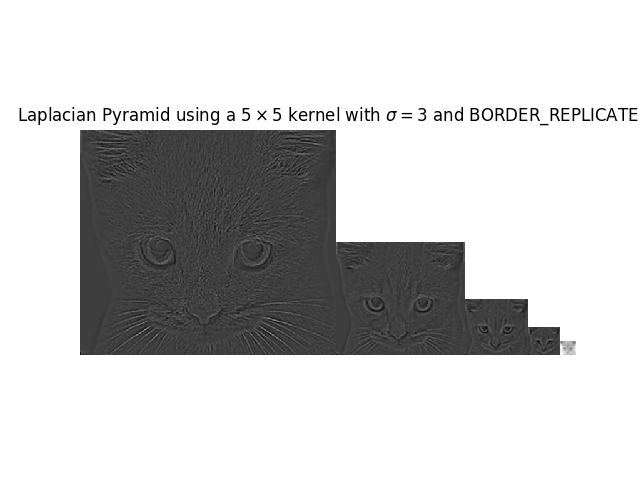
\includegraphics[scale=0.6]{img/lap-pyr-1.png}
\caption{Pirámide Laplaciana utilizando un \textit{kernel} $5 \times 5$ en cada nivel con $\sigma = 3$.}
\label{fig:lap-pyr-1}
\end{figure}

Se puede ver que los niveles bajos son los que tienen las frecuencias altas, mientras que el más alto (el último) es el
que contiene las frecuencias bajas de la imágen. De esta forma, se puede realizar una reconstrucción de la imágen sencilla
y conservando casi todos los detalles, cosa que con la pirámide Gaussiana no ocurría, ya que solo se almacenan las bajas
frecuencias.

De nuevo, tal y como hicimos antes, para ver qué efecto tiene cambiar el tipo de borde, vamos a probar a construir la misma
pirámide, pero cambiando a un borde de tipo constante. A continuación se puede ver la pirámide resultante:

\begin{figure}[H]
\centering
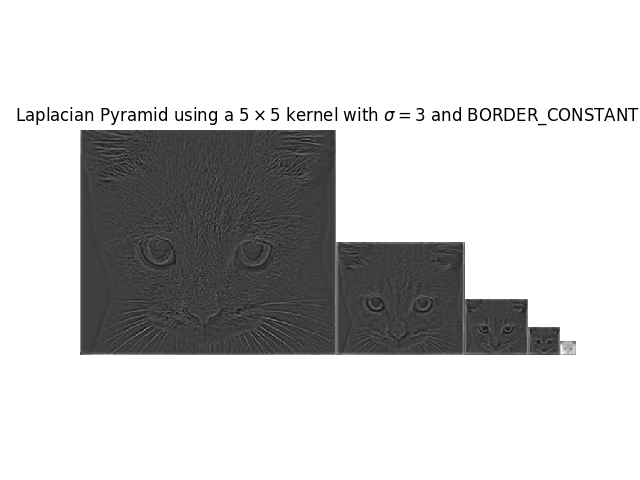
\includegraphics[scale=0.5]{img/lap-pyr-2.png}
\caption{Pirámide Laplaciana con tipo de borde constante.}
\label{fig:lap-pyr-2}
\end{figure}

Se puede ver que sí que existen ciertas diferencias si se compara con la figura \ref{fig:lap-pyr-1}. De nuevo, es como
si la imágen estuviese enmarcada, ya que empiezan a aparecer bordes, aunque esta vez son blancos en las imágenes de altas
frecuencias, y de forma menos visible pero aún así presente, negros en la imágen de baja frecuencia, tal y como sucedía en
la figura \ref{fig:gauss-pyr-2}. 

\subsection{Apartado C}

Para comenzar, vamos a ilustrar cuál es el código que realiza la función de obtener un espacio de escalas Laplaciano:

\begin{lstlisting}[caption={Función que crea un espacio de escalas Laplaciano},label={alg:lap-space-scale}]
def laplacian_scale_space(img, ksize, border, N, sigma=1.0, sigma_inc=1.2):
    """
    Funcion que construye el espacio de escalas Laplaciano de una imagen dada

    Args:
        img: Imagen de la que extraer el espacio de escalas
        ksize: Tamaño del kernel
        border: Tipo de borde
        N: Numero de escalas
        sigma: Valor inicial del kernel (default 1)
        sigma_inc: Multiplicador que incrementa el sigma (default 1.2)
    Return:
        Devuelve una lista con N imagenes, formando el espacio de escalas y los
        valores de sigma utilizados
    """
    # Crear listas que contendran las imagenes y los sigma
    scale_space = []
    sigma_list = []

    # Crear las N escalas
    for _ in range(N):
        # Aplicar Laplacian of Gaussian
        level_img = log_kernel(img, ksize, sigma, sigma, border)

        # Normalizar multiplicando por sigma^2
        level_img *= sigma ** 2

        # Elevar al cuadrado la imagen resultante
        level_img = level_img ** 2

        # Suprimir no maximos
        supressed_level = non_max_supression(level_img)

        # Guardar imagen y sigma
        scale_space.append(supressed_level)
        sigma_list.append(sigma)

        # Incrementar sigma
        sigma *= sigma_inc

    return scale_space, sigma_list
\end{lstlisting}

Esta función es bastante sencilla de entender. Se encarga de crear un espacio de escalas Laplaciano de $N$ niveles.
Para ello, partiendo siempre de la imágen original, aplica un filtro de Laplaciana de Gaussiana como el que se puede
ver en el algoritmo \ref{alg:log-kernel}. Después, normaliza la imágen multiplicando por $\sigma^2$ y, para eliminar
todos aquellos valores negativos, se eleva cada píxel de la imágen resultante al cuadrado. Acto seguido se suprimen
los no máximos y se guarda la imágen resultante. También se guarda el $\sigma$ utilizado, aunque esto es para ofrecer
información extra luego. Finalmente, se multiplica $\sigma$ por 1.2, y se repite todo el proceso.

Como se pude ver, por defecto, el valor de $\sigma$ inicial es 1, ya que no interesa aplicar mucho alisamiento al principio.
Adicionalemnte, el incremento por defecto de $\sigma$ es 1.2, ya que de esta forma se puede ver mejor como van evolucionando
las regiones relevantes.

Para la supresión de no máximos se ha utilizado la siguiente función:

\begin{lstlisting}[caption={Función que hace la supresión de no máximos.},label={alg:non-max-supression}]
def non_max_supression(img):
    """
    Funcion que realiza la supresion de no maximos dada una imagen de entrada

    Args:
        img: Imagen sobre la que realizar la supresion de no maximos
    Return:
        Devuelve una nueva imagen sobre la que se han suprimido los maximos
    """
    # Crear imagen inicial para la supresion de maximos (inicializada a 0)
    supressed_img = np.zeros_like(img)

    # Para cada pixel, aplicar una caja 3x3 para determinar el maximo local
    for i,j in np.ndindex(img.shape):
        # Obtener la region 3x3 (se consideran los bordes para que la caja
        # tenga el tamaño adecuado, sin salirse)
        region = img[max(i-1, 0):i+2, max(j-1, 0):j+2]

        # Obtener el valor actual y el maximo de la region
        current_val = img[i, j]
        max_val = np.max(region)

        # Si el valor actual es igual al maximo, copiarlo en la imagen de supresion
        # de no maximos
        if max_val == current_val:
            supressed_img[i, j] = current_val

    return supressed_img
\end{lstlisting}

Lo único que se realiza es crear una imágen nueva con todos los valores a 0, y se recorre la imágen sobre la que se
ha aplicado el filtro Laplaciana de Gaussiana normalizado y elevado al cuadrado. En cada caso se comprueba si el píxel
$(i, j)$, es decir, el actual, tiene el mismo valor que el máximo de la región. Para la región, se ha escogido un
tamaño de $3 \times 3$, porque es el que se escoge normalmente. En caso de que el píxel actual sea igual al máximo, se copia
su valor en la posición $(i, j)$ de la imágen resultante. En caso contrario, se deja a 0, ya que no es un máximo.

Puede que la línea que resulte más intrigante del algoritmo \ref{alg:non-max-supression} es la 17, donde se determina
la región. De la forma en la que se hace, nos aseguramos que en ningún momento nos salimos de las dimensiones de la
matriz que representa la imágen por la izquierda y por arriba, ya que no importa que nos pasemos de más por los extremos
de la derecha y por abajo. De esta forma, controlamos los bordes. En caso de no hacerlo así, obtendríamos un error por
problemas de indexación. No hace falta controlar que no nos salgamos de los otros bordes porque Numpy no da problemas
al pasarnos de tamaño, siempre y cuando alguno de los píxels de la imágen formen parte de esa región.

Una vez comentado esto, vamos a ver cómo sería aplicar esta función sobre nuestra imágen del gato. Para ello, vamos
a obtener un espacio de escalas con 5 escalas utilizando un \textit{kernel} de tamaño 5 y borde de replicado. Se ha
escogido este tamaño de máscara porque nos ha ofrecido unos buenos resultados en los apartados anteriores, y el borde
de replicado ofrece unos resultados razonables. El resto de parámetros ($\sigma$ e incremento) se dejan a los valores
por defecto por los motivos comentados anteriormente.

También se pide que, sobre estas escalas se dibujen círculos proporcionales a $\sigma$ de las regiones relevantes. Ya
que no se indica exactamente cómo hacerlo, vamos a suponer que aquellas regiones relevantes son las que tienen una intensidad
de gris superior a 128. Como tampoco se indica qué tamaño deben tener los círculos, vamos a suponer que tienen un radio de
$15\sigma$ según el $\sigma$ utilizado para la escala.

A continuación se pueden ver la imágen resultado de aplicarle la supresión de no máximos y la imágen con las regiones relevantes:

\begin{figure}[H]
\begin{subfigure}{.5\linewidth}
	\centering
	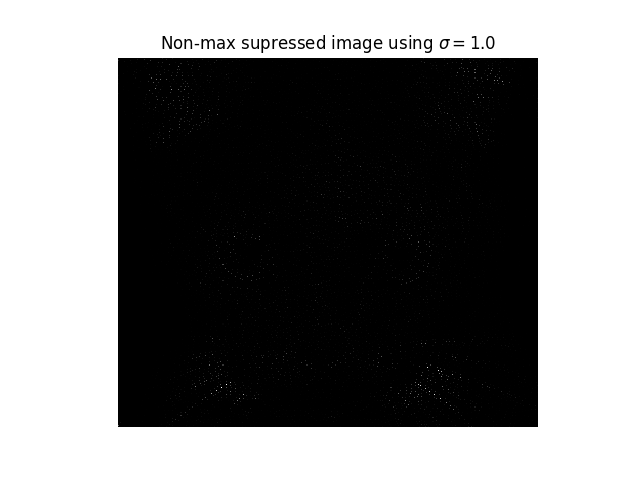
\includegraphics[scale=0.5]{img/non-max1.png}
	\caption{Supresión de no máximos del nivel 1.}
	\label{fig:non-max1}
\end{subfigure}
\begin{subfigure}{.5\linewidth}
	\centering
	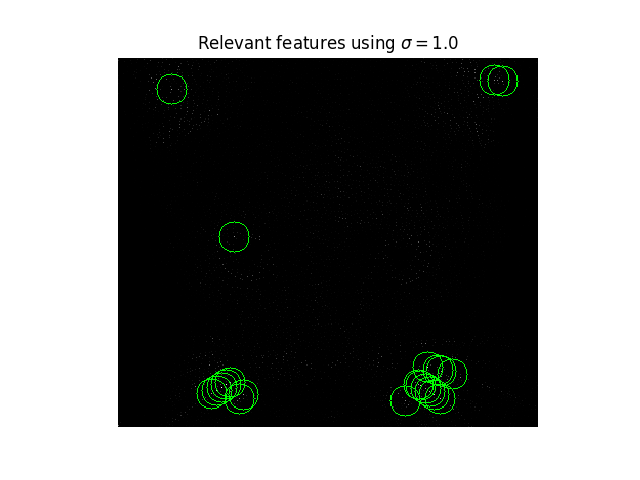
\includegraphics[scale=0.5]{img/features1.png}
	\caption{Regiones relevantes del nivel 1.}
	\label{fig:features1}
\end{subfigure}
\caption{Resultados del nivel 1 de escalas Laplaciano.}
\label{fig:lap-scale-space1}
\end{figure}

\begin{figure}[H]
\begin{subfigure}{.5\linewidth}
	\centering
	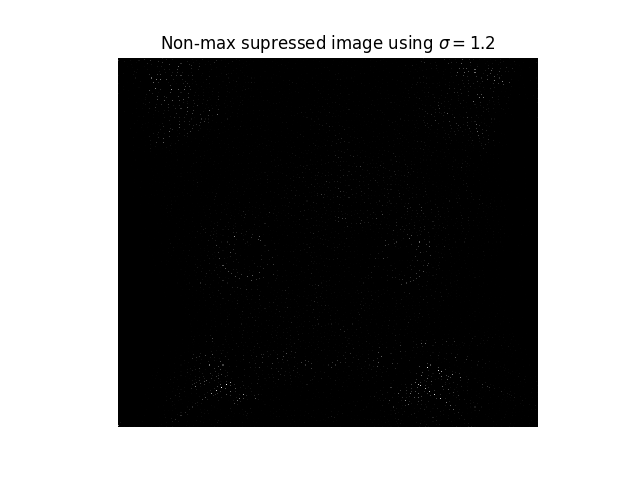
\includegraphics[scale=0.5]{img/non-max2.png}
	\caption{Supresión de no máximos del nivel 2.}
	\label{fig:non-max2}
\end{subfigure}
\begin{subfigure}{.5\linewidth}
	\centering
	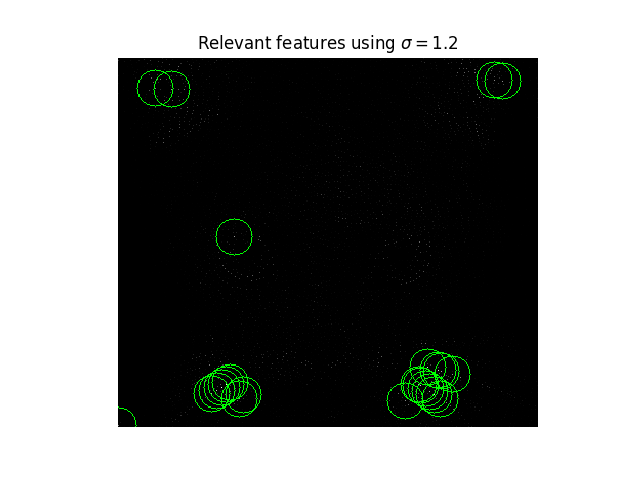
\includegraphics[scale=0.5]{img/features2.png}
	\caption{Regiones relevantes del nivel 2.}
	\label{fig:features2}
\end{subfigure}
\caption{Resultados del nivel 2 de escalas Laplaciano.}
\label{fig:lap-scale-space2}
\end{figure}

\begin{figure}[H]
\begin{subfigure}{.5\linewidth}
	\centering
	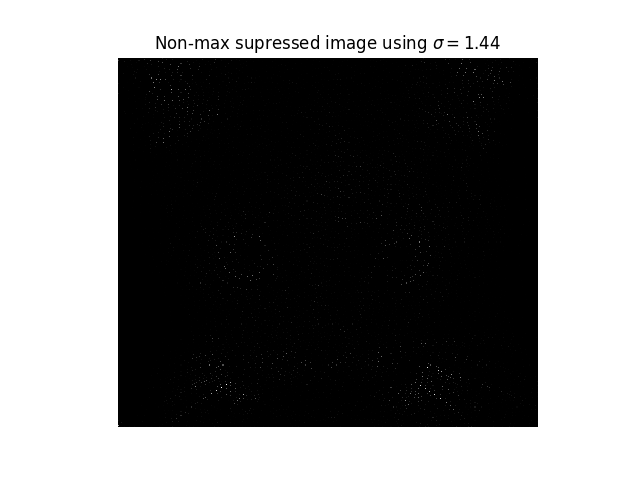
\includegraphics[scale=0.5]{img/non-max3.png}
	\caption{Supresión de no máximos del nivel 3.}
	\label{fig:non-max3}
\end{subfigure}
\begin{subfigure}{.5\linewidth}
	\centering
	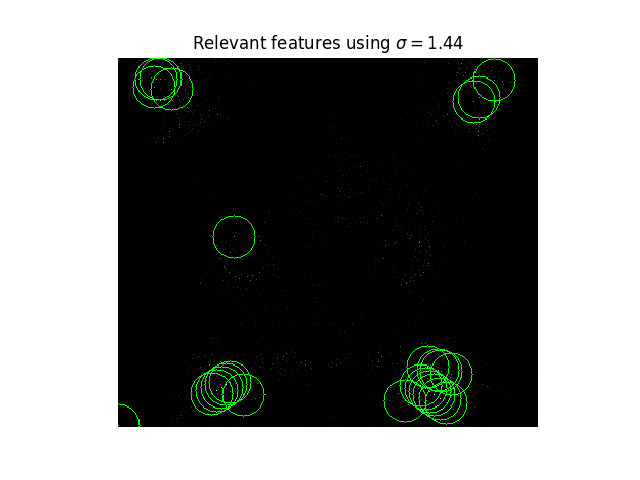
\includegraphics[scale=0.5]{img/features3.png}
	\caption{Regiones relevantes del nivel 3.}
	\label{fig:features3}
\end{subfigure}
\caption{Resultados del nivel 3 de escalas Laplaciano.}
\label{fig:lap-scale-space3}
\end{figure}

\begin{figure}[H]
\begin{subfigure}{.5\linewidth}
	\centering
	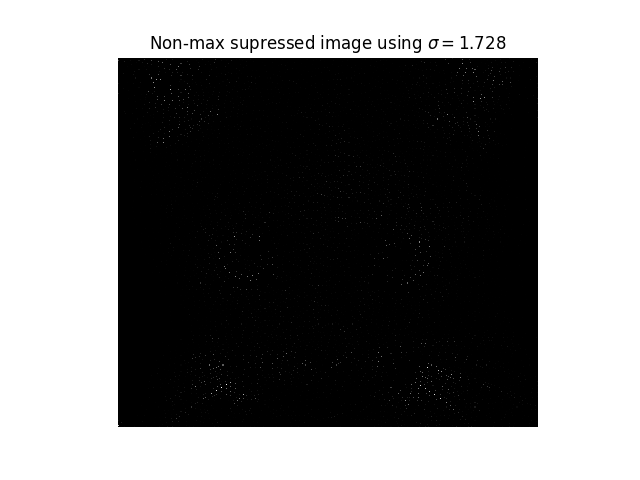
\includegraphics[scale=0.5]{img/non-max4.png}
	\caption{Supresión de no máximos del nivel 4.}
	\label{fig:non-max4}
\end{subfigure}
\begin{subfigure}{.5\linewidth}
	\centering
	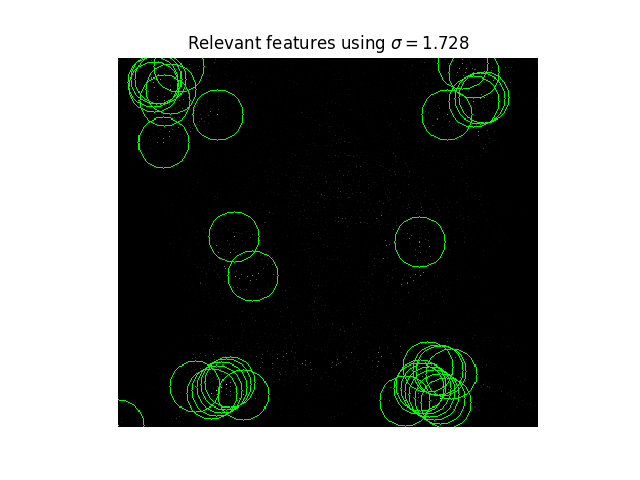
\includegraphics[scale=0.5]{img/features4.png}
	\caption{Regiones relevantes del nivel 4.}
	\label{fig:features4}
\end{subfigure}
\caption{Resultados del nivel 4 de escalas Laplaciano.}
\label{fig:lap-scale-space4}
\end{figure}

\begin{figure}[H]
\begin{subfigure}{.5\linewidth}
	\centering
	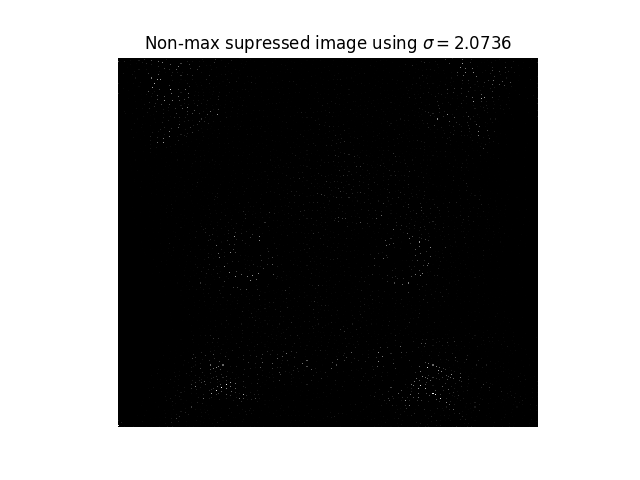
\includegraphics[scale=0.5]{img/non-max5.png}
	\caption{Supresión de no máximos del nivel 5.}
	\label{fig:non-max5}
\end{subfigure}
\begin{subfigure}{.5\linewidth}
	\centering
	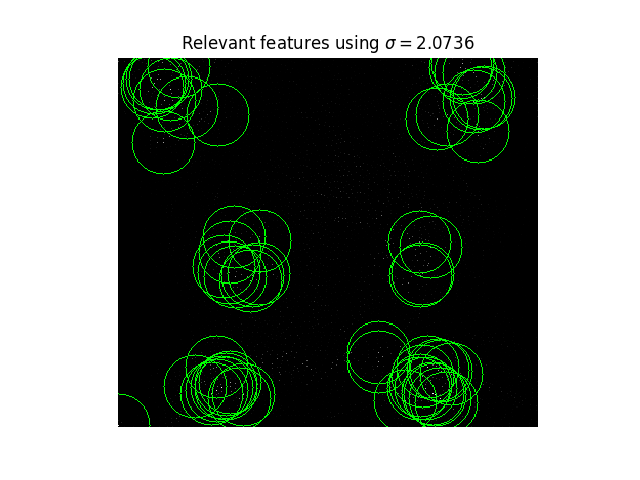
\includegraphics[scale=0.5]{img/features5.png}
	\caption{Regiones relevantes del nivel 5.}
	\label{fig:features5}
\end{subfigure}
\caption{Resultados del nivel 5 de escalas Laplaciano.}
\label{fig:lap-scale-space5}
\end{figure}

Como se puede ver, a medida que va aumentando el valor de $\sigma$ el número de regiones relevantes se va incrementando.
Esto puede deberse a que al incrementar el valor de $\sigma$ se suaviza más, y por tanto, los píxels comienzan a tener
unos valores más similares.

Puede que este incremento de regiones no se vea muy nítido en el documento debido al tamaño de las figuras y a la compresión
que se hace de las imágenes, pero si nos fijamos en las regiones de los ojos, las orejas y los bigotes, podemos ver que se van
``encendiendo'' más píxels. Esto se pone de manifiesto con la cantidad de círculos nuevos que van apareciendo en estas zonas,
ya que a medida que aumenta el $\sigma$ van apareciendo más y más.

\newpage

\section{\textsc{Imágenes híbridas}}

\noindent \textbf{Mezclando adecuadamente una parte de las frecuencias altas de una imagen con una parte de
las frecuencias bajas de otra imagen, obtenemos una imagen híbrida que admite distintas interpretaciones a distintas
distancias (ver hybrid images project page).}

\noindent \textbf{Para seleccionar la parte de frecuencias altas y bajas que nos quedamos
de cada una de las imágenes usaremos el parámetro sigma del núcleo/máscara de alisamiento gaussiano que usaremos.
A mayor valor de sigma mayor eliminación de altas frecuencias en la imagen convolucionada. Para una buena
implementación elegir dicho valor de forma separada para cada una de las dos imágenes (ver las recomendaciones
dadas en el paper de Oliva et al.). Recordar que las máscaras 1D siempre deben tener de longitud un número impar.}

\noindent \textbf{Implementar una función que genere las imágenes de baja y alta frecuencia a partir de las
parejas de imágenes (solo en la versión de imágenes de gris). El valor de sigma más adecuado para cada pareja
habrá que encontrarlo por experimentación.}

\begin{enumerate}
	\item Escribir una función que muestre las tres imágenes (alta, baja e híbrida) en una misma ventana.
	(Recordar que las imágenes después de una convolución contienen número flotantes que pueden ser positivos y negativos)
	\item Realizar la composición con al menos 3 de las parejas de imágenes
	\item Construir pirámides gaussianas de al menos 4 níveles con las imágenes resultado. Explicar el efecto que se observa.
\end{enumerate}

\subsection{Apartado 1}

En este apartado se ha pedido crear las funciones. Por tanto, en el siguiente apartado veremos las composiciones
que se han creado. Así que, de momento, vamos a echarle un vistazo a la función que permite crear las imágenes híbridas:

\begin{lstlisting}[caption={Función que crea imágenes híbridas.},label={alg:hybrid-img}]
def hybrid_image_generator(img_low, img_high, ksize, sigma_low, sigma_high, border):
    """
    Funcion que permite crear una imagen hibrida combinando dos imagenes

    Args:
        img_low: Imagen que sera utilizada para las bajas frecuencias
        img_high: Imagen que sera utilizada para las altas frecuencias
        ksize: Tamaño del kernel (es una tupla)
        sigma_low: Sigma para la imagen de bajas frecuencias
        sigma_high: Sigma para la imgane de altas frecuencias
        border: Tipo de borde
    Return:
        Devuelve una lista que contiene la imagen de bajas frecuencias, la de altas
        y la hibrida
    """
    # Crear la imagen de bajas frecuencias aplicando filtro Gaussiano
    low_freq_img = gaussian_kernel(img_low, ksize, ksize, sigma_low, sigma_low, border)

    # Crear imagen de altas frecuencias aplicando filtro Gaussiano y restando a la original
    gauss_high_freq = gaussian_kernel(img_high, ksize, ksize, sigma_high, sigma_high, border)
    high_freq_img = img_high - gauss_high_freq

    # Crear la imagen hibrida combinando las dos
    hybrid = low_freq_img + high_freq_img

    return [low_freq_img, high_freq_img, hybrid]
\end{lstlisting}

Esta función crea la imágen híbrida con las frecuencias bajas de la primera y las altas de la segunda imágen que se le pasa.
Junto a esta, obtiene también las imágenes de bajas y altas frecuencias que se utilizan para componer la híbrida.
Para obtener las frecuencias bajas, basta con simplemente pasar un filtro Gaussiano. Para las altas, solo tenemos que obtener
las frecuencias bajas y restárselo a la imágen original, obteniendo por tanto las frecuencias altas. Finalmente, solo hace
falta combinar las dos imágenes resultantes en una sumándolas. De esta forma, se obtiene una imágen híbrida, compuesta
por las altas frecuencias de una de las imágenes y las altas de la otra.

Para visualizarlas, se ha creado la siguiente función:

\begin{lstlisting}[caption={Función que muestra múltiples imágenes en la misma ventana.},label={alg:vis-mult}]
def visualize_mult_images(images, titles=None):
    """
    Funcion que pinta multiples imagenes en una misma ventana. Adicionalmente
    se pueden especificar que titulos tendran las imagenes.

    Args:
        images: Lista con las imagenes
        titles: Titulos que tendran las imagenes (default None)
    """

    # Obtener el numero de imagenes
    n_img = len(images)

    # Crear n_cols sublots (un subplot por cada imagen)
    # El formato sera 1 fila con n_cols columnas
    _, axarr = plt.subplots(1, n_img)

    # Pintar cada imagen
    for i in range(n_img):
        # Convertir la imagen a uint8
        img = transform_img_uint8(images[i])

        # Pasarla de BGR a RGB
        img = cv.cvtColor(img, cv.COLOR_BGR2RGB)

        # Obtener siguiente imagen
        axarr[i].imshow(img)

        # Determinar si hay que poner o no titulo
        if titles != None:
            axarr[i].set_title(titles[i])

        axarr[i].axis('off')

    # Mostar imagenes
    plt.show()
\end{lstlisting}

Para mostrarlas, las imágenes se pasan primero a \textit{uint8} (hace falta recordar que hemos estado trabajando con
imágenes en \textit{float64} hasta ahora). Además, ya que se está usando el módulo \textit{matplotlib}, se tiene
que cambiar del formato BGR (el que usa OpenCV) a RGB (el que utiliza el módulo mencionado anteriormente). Hace falta recalcar
que esto se ha hecho con todas las imágenes hasta ahora, y no es exlusivo de las imágenes híbridas. Lo que sí que es
diferente es la forma en la que se dibujan, ya que hay que partir el \textit{plot} que se utiliza en tantos
\textit{subplots} como imágenes se quieran pintar a la vez.

\subsection{Apartado 2}

Una vez vistas las funciones, vamos a ver las composiciones creadas. Hace falta destacar que los valores de $\sigma$ que
se utilizan para la imágen de las altas frecuencias y para la de las bajas dependen mucho del par de imágenes, y se han
obtenido mediante experimentación.

Se han realizado las composiciones de todas las parejas de imágenes, las cuáles pueden ser vistas a continuación:

\begin{figure}[H]
\centering
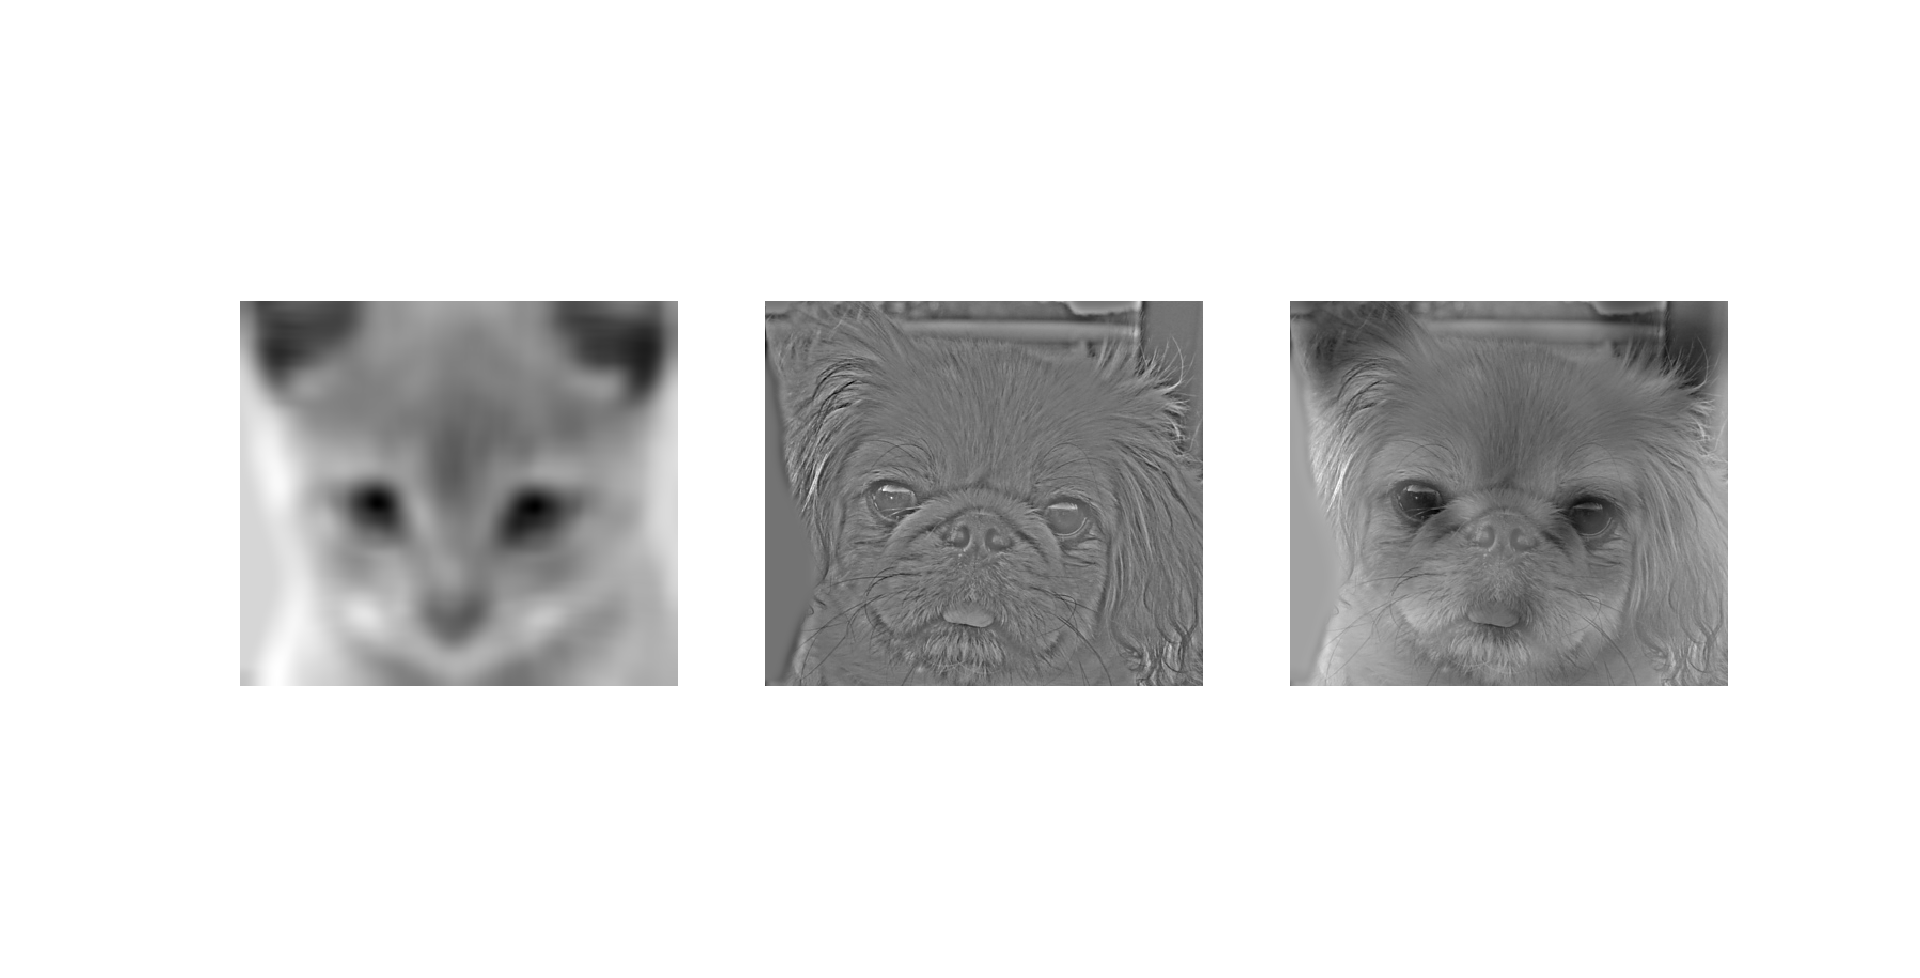
\includegraphics[scale=0.3]{img/hyb1.png}
\caption{Composición gato-perro.}
\label{fig:hyb1}
\end{figure}

\begin{figure}[H]
\centering
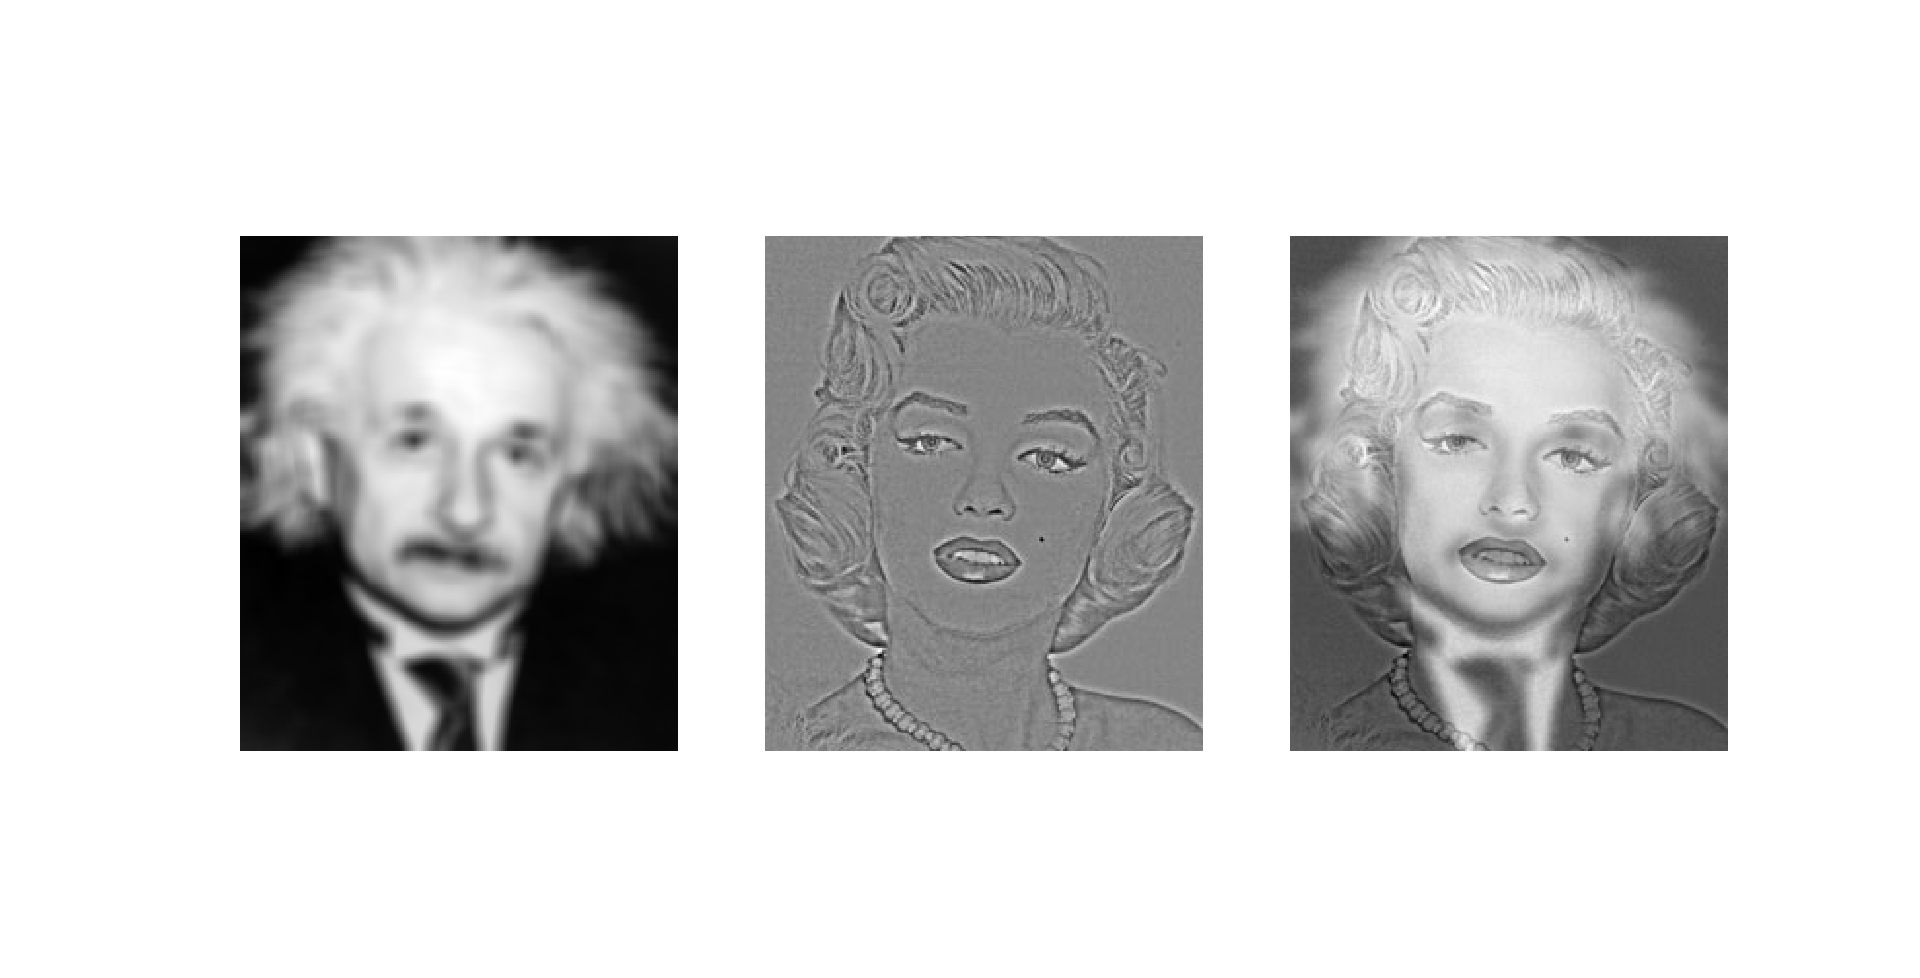
\includegraphics[scale=0.3]{img/hyb2.png}
\caption{Composición Einstein-Marilyn.}
\label{fig:hyb2}
\end{figure}

\begin{figure}[H]
\centering
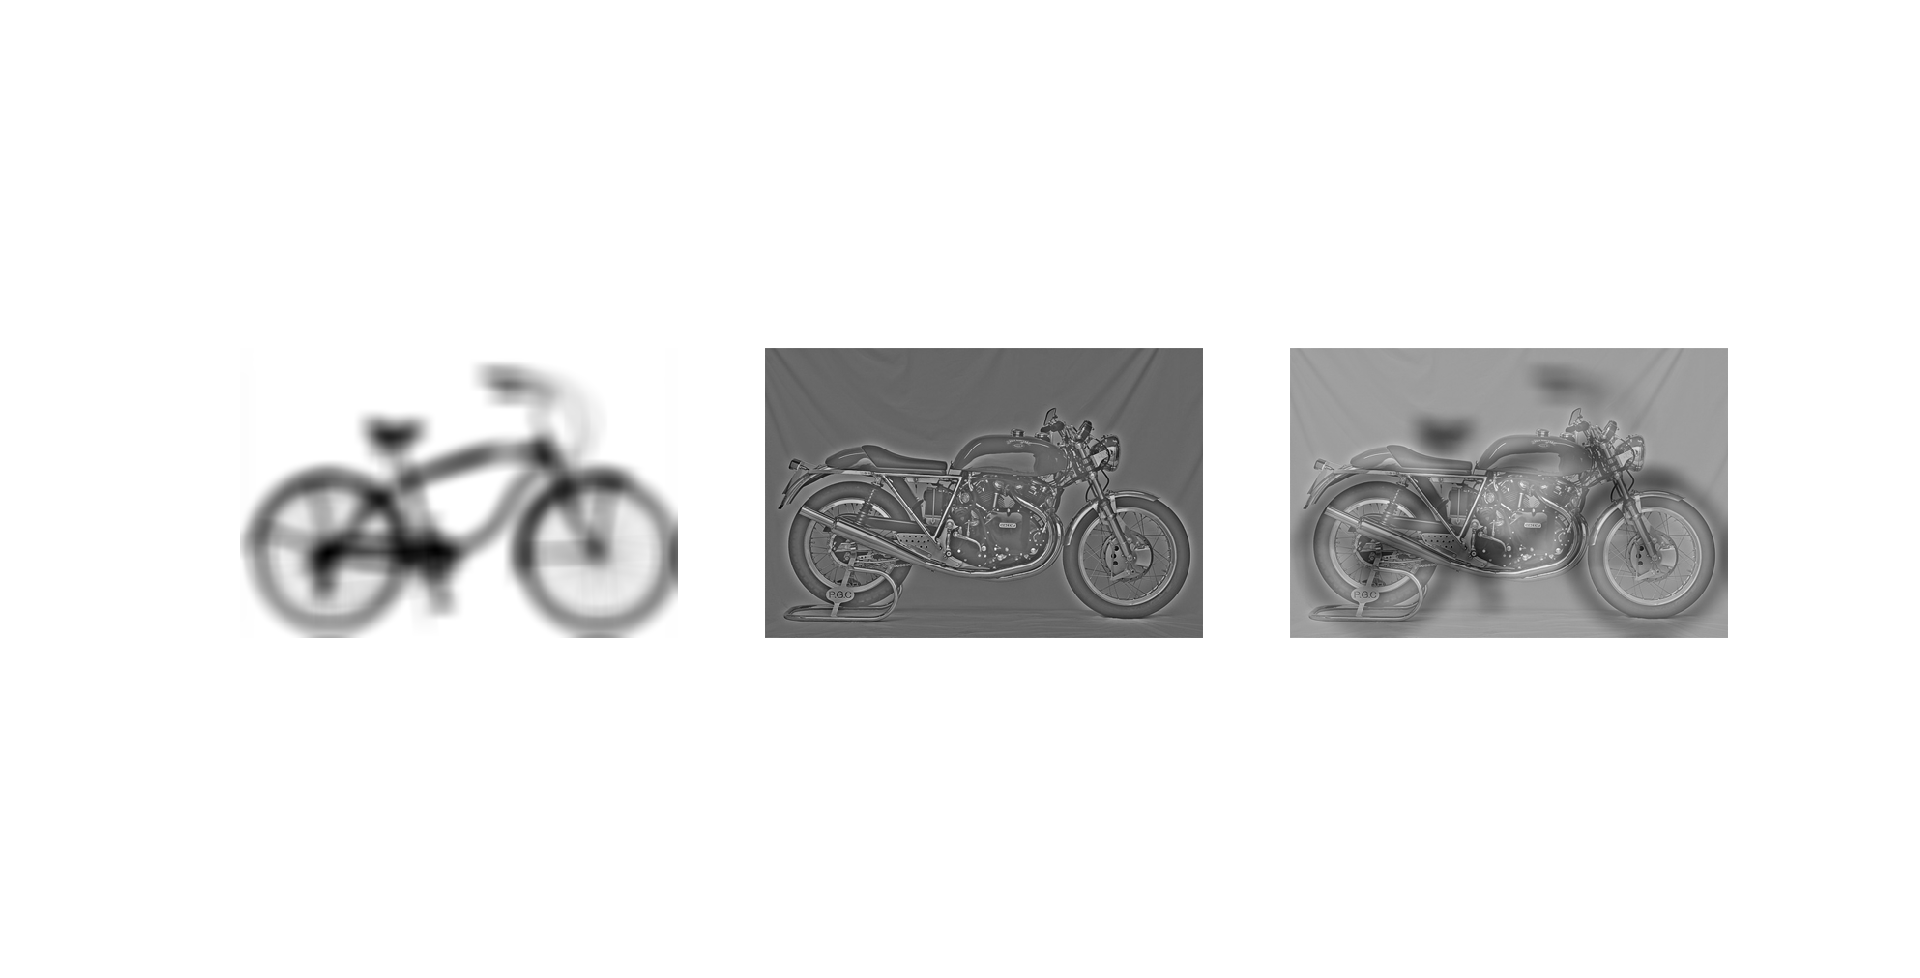
\includegraphics[scale=0.3]{img/hyb3.png}
\caption{Composición bicicleta-moto.}
\label{fig:hyb3}
\end{figure}

\begin{figure}[H]
\centering
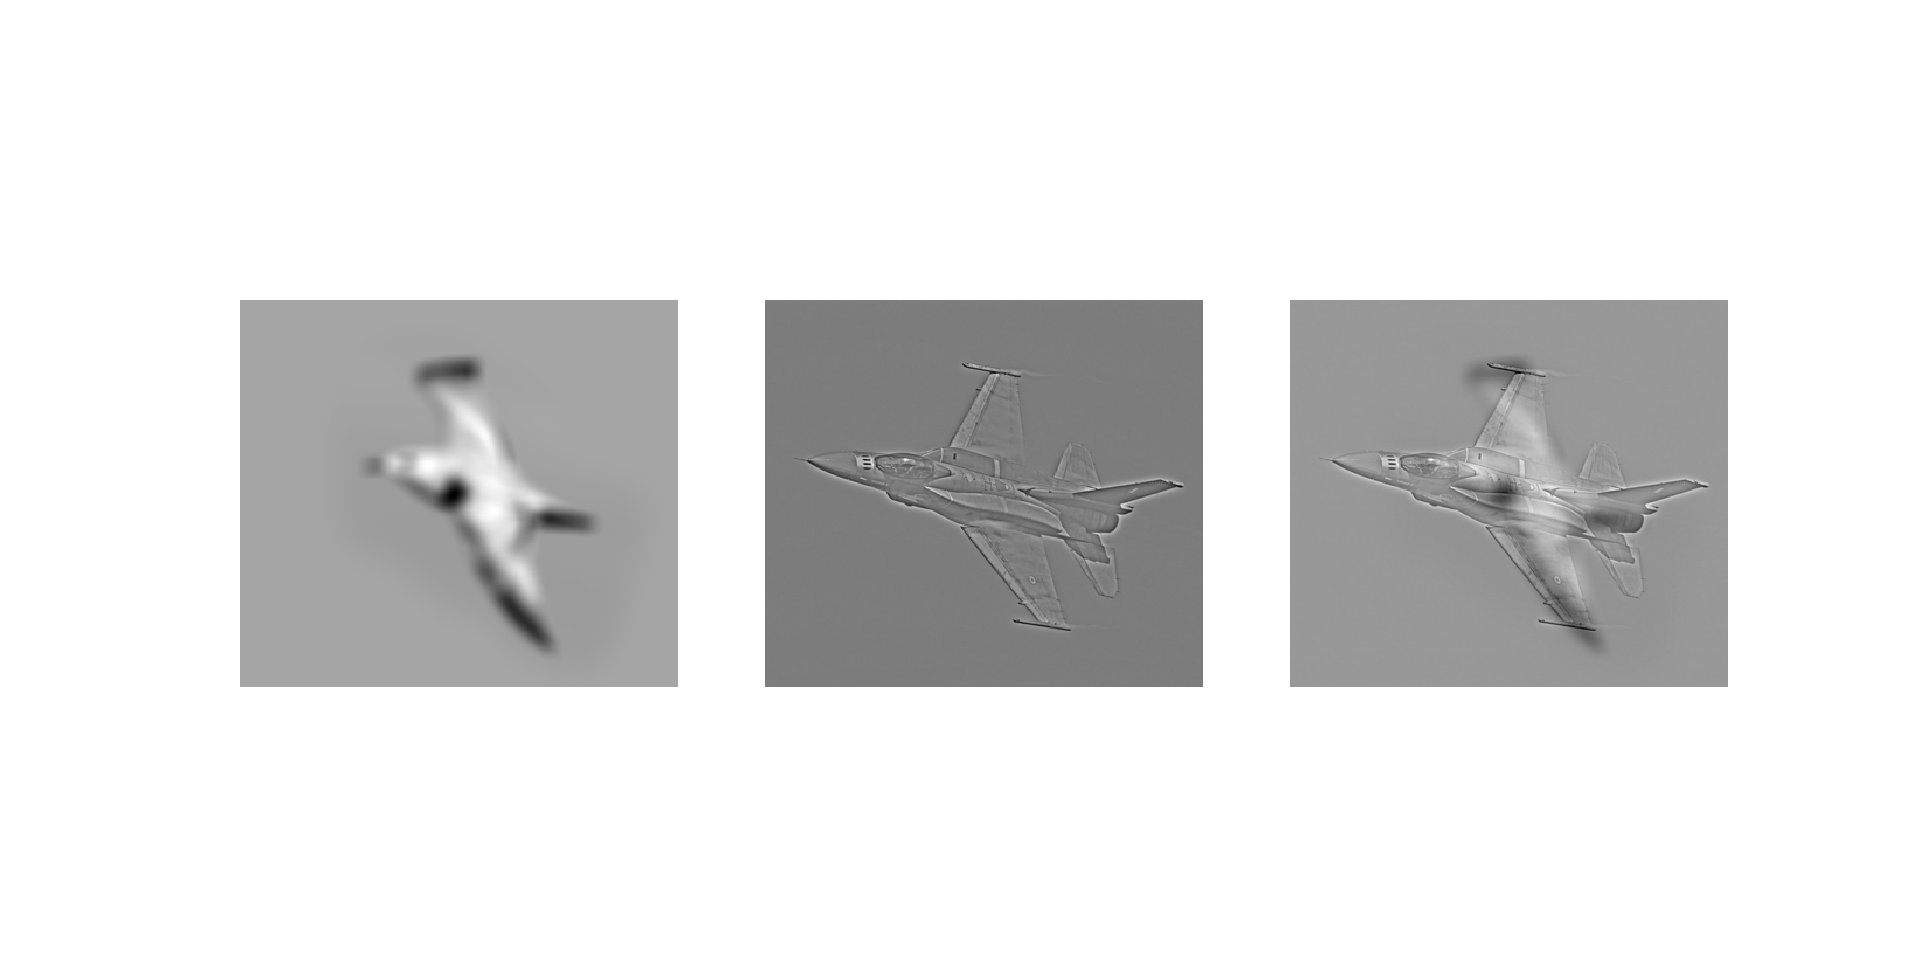
\includegraphics[scale=0.3]{img/hyb4.png}
\caption{Composición ave-avión.}
\label{fig:hyb4}
\end{figure}

\begin{figure}[H]
\centering
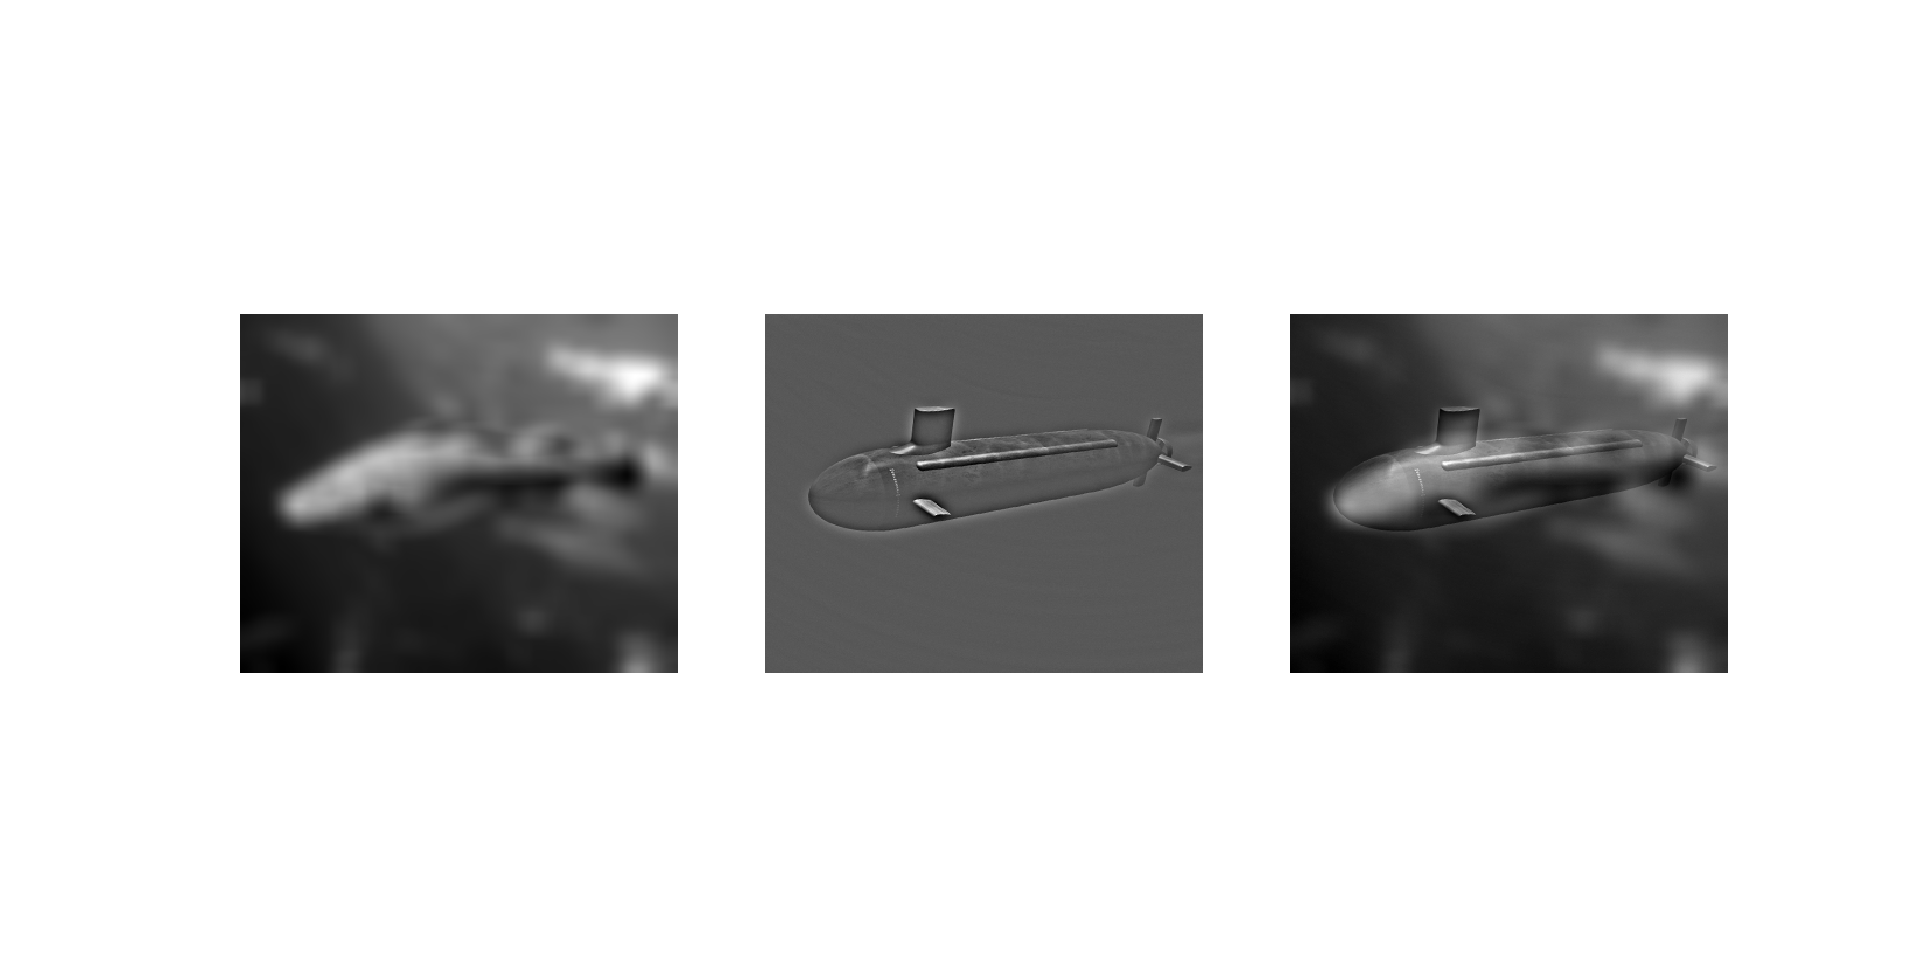
\includegraphics[scale=0.3]{img/hyb5.png}
\caption{Composición pez-submarino.}
\label{fig:hyb5}
\end{figure}

En la parte izquierda de cada figura se puede ver la imágen en bajas frecuencias que se ha utilizado. En la parte central
aparece la imágen de altas frecuencias. A la derecha se puede ver la imágen híbrida. En general, las imágenes híbridas
han quedado bastante bien, ya que se puede ver que la imágen de altas frecuencias es más distinguible de cerca
que la de bajas. Al revés pasaría lo mismo; ya que al alejarnos de la imágen, solo veríamos las bajas, y no las altas.

\subsection{Apartado 3}

En este apartado, vamos a simular que nos estamos alejando de la imágen para ver si podemos dejar de ver las altas
frecuencias. Para ello, en vez de tener que alejarnos nosotros de la pantalla, podemos ir disminuyendo el tamaño de la
imágen híbrida para ver cómo va cambiando lo que vemos a medida que nos vamos alejando. Aquí es donde entra en juego la pirámide
Gaussiana, la cuál permite visualizar esta evolución de forma sencilla, ya que incluye versiones más grandes de la
imágen y más pequeñas.

Para construir la pirámide, se ha utilizado un $N=4$ (es decir, que se verán 4 imágenes en la pirámide), con un tamaño de
\textit{kernel} de 5 y un $\sigma=3$ para cada eje, tal y como se ha hecho en los apartados anteriores.
Para el tipo de borde, se ha elegido de nuevo el borde de replicado.

A continuación se pueden ver ejemplos de las pirámides Gaussianas:

\begin{figure}[H]
\centering
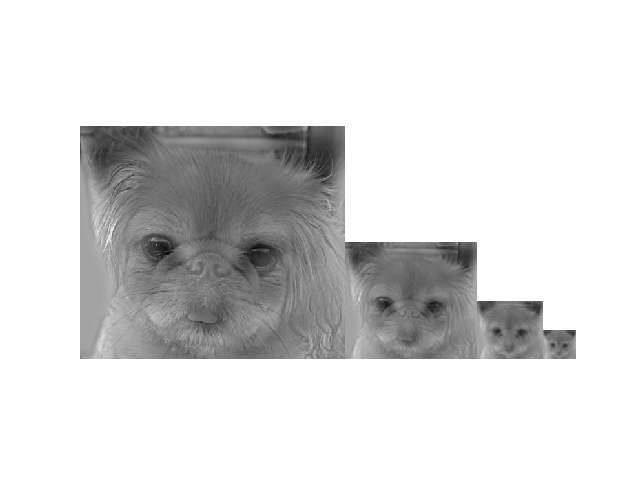
\includegraphics[scale=0.7]{img/hyb-pyr1.png}
\caption{Pirámide Gaussiana de la composición gato-perro.}
\label{fig:hyb-pyr1}
\end{figure}

\begin{figure}[H]
\centering
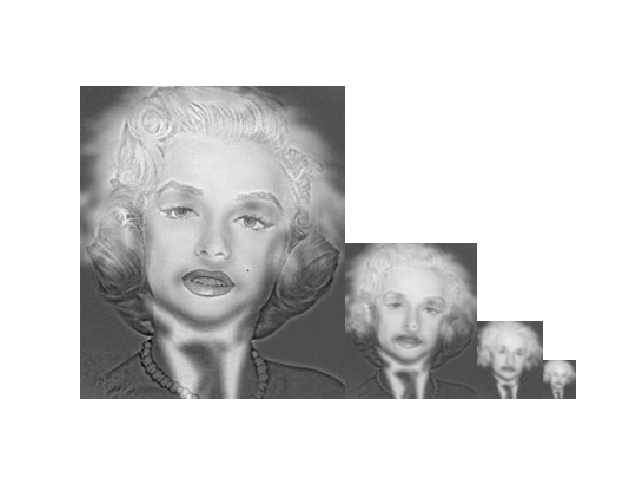
\includegraphics[scale=0.7]{img/hyb-pyr2.png}
\caption{Pirámide Gaussiana de la composición Einstein-Marilyn.}
\label{fig:hyb-pyr2}
\end{figure}

\begin{figure}[H]
\centering
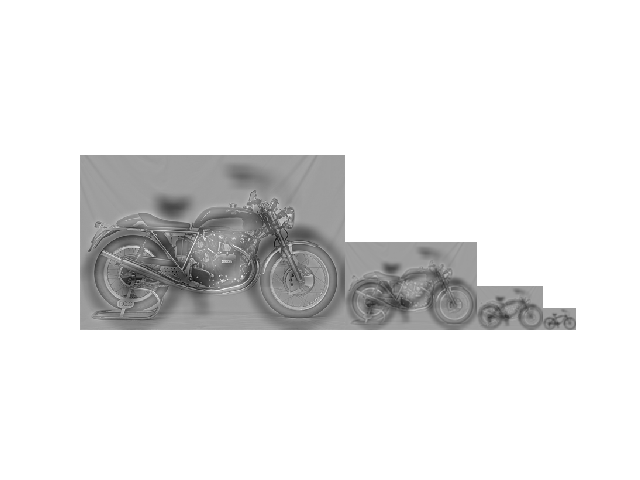
\includegraphics[scale=0.7]{img/hyb-pyr3.png}
\caption{Pirámide Gaussiana de la composición bicicleta-moto.}
\label{fig:hyb-pyr4}
\end{figure}

\begin{figure}[H]
\centering
\includegraphics[scale=0.7]{img/hyb-pyr4.png}
\caption{Pirámide Gaussiana de la composición ave-avión.}
\label{fig:hyb-pyr4}
\end{figure}

\begin{figure}[H]
\centering
\includegraphics[scale=0.7]{img/hyb-pyr5.png}
\caption{Pirámide Gaussiana de la composición pez-submarino.}
\label{fig:hyb-pyr5}
\end{figure}

Como se puede ver, a medida que se va haciendo más pequeña la imágen, menos se ve la parte de imágen que tiene frecuencias
altas, hasta que al final solo se ve la imágen de bajas frecuencias. Esto se debe a que las ondas de frecuencia alta
viajan una menor distancia en el espacio debido a que tienen una menor amplitud de onda. Las frecuencias bajas,
en cambio, tienen una amplitud de onda mayor, y son capaces de recorrer una mayor distancia. De esta forma, a medida
que nos alejamos o reducimos el tamaño de la imágen, menos altas frecuencias nos van a llegar, hasta que al final solo
nos lleguen las bajas, tal y como se ha dicho anteriormente.

\newpage

\section{\textsc{Bonus}}

\subsection{Convolución 2D propia}

\noindent \textbf{Implementar con código propio la convolución 2D con cualquier máscara 2D de números reales usando
máscaras separables.}

Para esta sección se han hecho dos cosas:

\begin{enumerate}
	\item Implementar la correlación 1D con código propio.
	\item Implementar la convolución 2D utilizando la correlación 1D implementada anteriormente.
\end{enumerate}

Vamos a comenzar explicando la correlación 1D. Se ha implementado el siguiente código:

\begin{lstlisting}[caption={Función que realiza la correlación 1D},label={alg:corr-1d}]
def correlation_1D(img, kernel):
    """
    Funcion que aplica la correlacion 1D sobre una imagen de entrada utilizando
    un kernel dado

    Args:
        img: Imagen sobre la que aplicar la correlacion
        kernel: Kernel que se aplicara
    Return:
        Devuelve una imagen sobre la que se ha aplicado correlacion 1D por filas
    """
    # Obtener el numero de elementos que se deben replicar al principio y al final
    # de la imagen
    n_replica = kernel.shape[0] // 2

    # Replicar elemento inicial y final de la imagen n_replica veces
    replica_img = np.hstack([np.tile(img[:, 0].reshape(-1, 1), n_replica), img])
    replica_img = np.hstack([replica_img, np.tile(img[:, -1].reshape(-1, 1), n_replica)])

    # Crear matriz de salida con el mismo tamaño que img
    correlation_mat = np.empty_like(img)

    # Aplicar la correlacion sobre cada elemento (i, j) de la imagen
    for i in range(img.shape[0]):
        for j in range(n_replica, img.shape[1] + n_replica):
            # Obtener sub imagen del mismo tamaño que el kernel
            sub_img = replica_img[i, j - n_replica:j + n_replica + 1]

            # Realizar producto escalar de la sub imagen y el kernel
            corr_value = np.dot(sub_img, kernel)

            # Actualizar valor de la matriz de correlacion
            correlation_mat[i, j - n_replica] = corr_value

    return correlation_mat
\end{lstlisting}

Vamos a ir explicando lo que hace el código para que se entienda cuál es la idea general. Lo primero que hay que
hacer es extender la imágen que se pasa como argumento, de modo que tenga más píxels. Esto se hace por los bordes, debido
a que también se tiene que calcular la correlación ahí y, en caso de no tener más valores más allá de ellos, se estaría
haciendo un cálculo incorrecto. Para ello, se replica el píxel del borde un número de veces. Este número de veces
está determinado por la variable $n\_replica$, la cuál viene dada por la siguiente expresión:

\begin{equation}
	n\_replica = \floor*{\frac{KernelSize}{2}}
\end{equation}

Esto se debe a que los \textit{kernels} tienen un tamaño impar, debido a que consideran $KernelSize \; / \; 2 - 1$ vecinos
a cada lado del píxel $(i, j)$ de la imágen. Este píxel (el cuál es el central del \textit{kernel}) hace que el tamaño
de la máscara sea siempre impar. Por tanto, nos interesa saber cuántas veces tenemos que replicar el borde de la imágen según el
tamaño del \textit{kernel} que se le pase.

Se ha elegido hacer un replicado debido a que no estaba nada especificado en el enunciado del ejercicio, además de que
es lo más sencillo de hacer. Por tanto, lo que se hace es copiar el primer y el último píxel de cada fila de la imágen
$n\_replica$ veces, tal y como hace el tipo de borde $BORDER\_REPLICATE$ de OpenCV. Este replicado se puede ver en las
líneas 17 y 18 del código \ref{alg:corr-1d}, donde se crea una nueva matriz en la que se concatenan primero al principio
y luego al final las réplicas del primer y del último píxel de la imágen original, respectivamente. Esta operación está
vectorizada, por tanto, se hace para todas las filas a la vez.

Después, se crea una matriz de salida, $correlation\_mat$, la cuál tiene las mismas dimensiones que la imágen de entrada.
Aquí es dónde se escribirá el resultado de la convolución. A continuación se recorren todas las filas de la de la imágen
replicada, lo cuál se corresponde con la línea 24. La imágen replicada tiene el mismo número de filas que la original, así que
usaremos el número de filas de la original para delimitar el rango del bucle, por comodidad más que nada. Para cada fila,
se comienza a partir de columna $n\_replica$, debido a que queremos dejar tantos vecinos a la izquierda del píxel
central inicial, y se recorre la imágen replicada hasta la columna $NumColumnasImagenOriginal + n\_replica$, aplicando
la correlación. De esta forma, recorremos la imágen original dentro de la replicada, y usamos los píxeles replicados solo
para el cálculo de la correlación. Ninguno de estos píxels replicados estará en el centro de la correlación por las condiciones
especificadas anteriormente.

Para el cálculo de la correlación, simplemente obtenemos una parte de la imágen del mismo tamaño que el \textit{kernel}
utilizando los índices definidos anteriormente, se realiza el producto escalar entre esta parte de la imágen y el \textit{kernel}
y se guarda el resultado en la matriz de salida. Es importante destacar que esta función asume que el \textit{kernel} viene
dado como un vector columna, para así poder realizar el producto escalar entre un vector fila (la parte de la imágen) y un
vector columna (el \textit{kernel}).

Ahora ya solo nos queda ver como se haría la convolución. A continuación se puede ver el código implementado:

\begin{lstlisting}[caption={Función que aplica la convolución 2D sobre una imágen.},label={alg:convolution}]
def convolution(img, kernel_x, kernel_y):
    """
    Funcion que aplica la convolucion sobre una imagen dados un kernel para
    el eje X y el eje Y
    
    Args:
        img: Imagen sobre la que aplicar la convolucion
        kernel_x: Kernel en el eje X
        kernel_y: Kernel en el eje Y
    Return:
        Devuelve la convolucion de la imagen con los kernels de entrada
    """
    # Hacer que los kernels sean vectores columna
    kernel_x = kernel_x.reshape(-1, 1)
    kernel_y = kernel_y.reshape(-1, 1)
    
    # Realizar un flip sobre los kernels
    kernel_x_flip = np.flip(kernel_x)
    kernel_y_flip = np.flip(kernel_y)

    # Realizar la convolucion (primero sobre el eje X y luego sobre el eje Y)
    convolution = correlation_1D(img, kernel_x_flip)
    convolution = correlation_1D(convolution.T, kernel_y_flip)

    # Trasponer la convolucion (porque se han cambiado filas por columnas anteriormente)
    convolution = convolution.T

    return convolution
\end{lstlisting}

Lo primero que se hace es transformar los \textit{kernels} de entrada para que sean vectores columna (si no lo eran ya). A
continuación, para poder aplicar la convolución hace falta realizar un \textit{flip} sobre los \textit{kernels} (líneas 18-19).
Como son vectores y no matrices, simplemente basta con darles la vuelta. Si no se hiciese, se aplicaría una correlación en vez de
una convolución, lo cuál no produciría el resultado deseado.

Una vez hecho esto, es el momento de aplicar la correlación utilizando los \textit{kernels} sobre los que se ha aplicado un
\textit{flip}. Primero se aplica sobre el eje X, lo cuál se puede ver en la línea 22 y no supone ningún problema. Sin embargo,
si nos damos cuenta de una cosa, la correlación 1D que se puede ver en el código \ref{alg:corr-1d} se aplica por filas. Para
aplicarla a las columnas, simplemente basta realizar la traspuesta de la imágen sobre la que se quiere realizar la correlación.
De esta forma, se cambiarán las filas por las columnas, y se podrá aplicar sin problema. Lo único que hará falta es trasponer
la imágen resultado al final, ya que tiene las filas y las columnas cambiadas. Esto se puede ver en la línea 26.

Para probar nuestra función, hemos aplicado un \textit{kernel} Gaussiano de $\sigma=3$ en cada eje y tamaño de \textit{kernel}
5 sobre la imágen del gatito que hemos estado usando hasta ahora. También hemos aplicado un filtro de primera derivada
en el eje $X$ con tamaño de \textit{kernel} 5. A continuación se pueden ver los resultados:

\begin{figure}[H]
\begin{subfigure}{.5\linewidth}
	\centering
	\includegraphics[scale=0.5]{img/conv1.png}
	\subcaption{Filtro Gaussiano.}
	\label{fig:conv1}
\end{subfigure}
\begin{subfigure}{.5\linewidth}
	\centering
	\includegraphics[scale=0.5]{img/conv2.png}
	\subcaption{Filtro de primera derivada.}
	\label{fig:conv2}
\end{subfigure}
\caption{Distintos filtros utilizando la convolución propia.}
\label{fig:conv}
\end{figure}

El código anteriormente mostrado funciona perfectamente ya que, como se puede comprobar, los resultados son los mismos que los
que se pueden ver para las figuras \ref{fig:gauss-sigma2} y \ref{fig:der-x1}.

\subsection{Imágenes híbridas a color}

\noindent \textbf{Realizar todas las parejas de imágenes híbridas en su formato a color (solo se tendrá en cuenta
si la versión de gris es correcta).}

\subsection{Imágen híbrida propia}

\noindent \textbf{Realizar una imagen híbrida con al menos una pareja de imágenes de su elección que hayan
sido extraídas de imágenes más grandes. Justifique la elección y todos los pasos que realiza.}

\newpage

\begin{thebibliography}{5}

\bibitem{nombre-referencia}
Texto referencia
\\\url{https://url.referencia.com}

\end{thebibliography}

\end{document}

